
\subsection{Flächenberechnung mit Ober- und Untersummen}
\subsubsection{Einführungsaufgaben}
Fragestellung: Wie bestimmt man den Flächeninhalt eines Gebietes, dessen Rand eine „gekrümmte Linie“ ist?
\begin{center}
	\includegraphics{media/flächeAllgemein.png}
\end{center}
Um uns an die Lösung dieses Problems zu nähern, reduzieren wir zunächst ein wenig die Schwierigkeit: Gegeben sei eine Funktion $f$, und ein Intervall $[a,b]$. Wir betrachten nun das Gebiet, das durch den Graphen von $f$, die $x$-Achse und die Geraden $x=a$ und $x=b$ berandet wird. Wie gross ist der Flächeninhalt $A$?
\begin{center}
	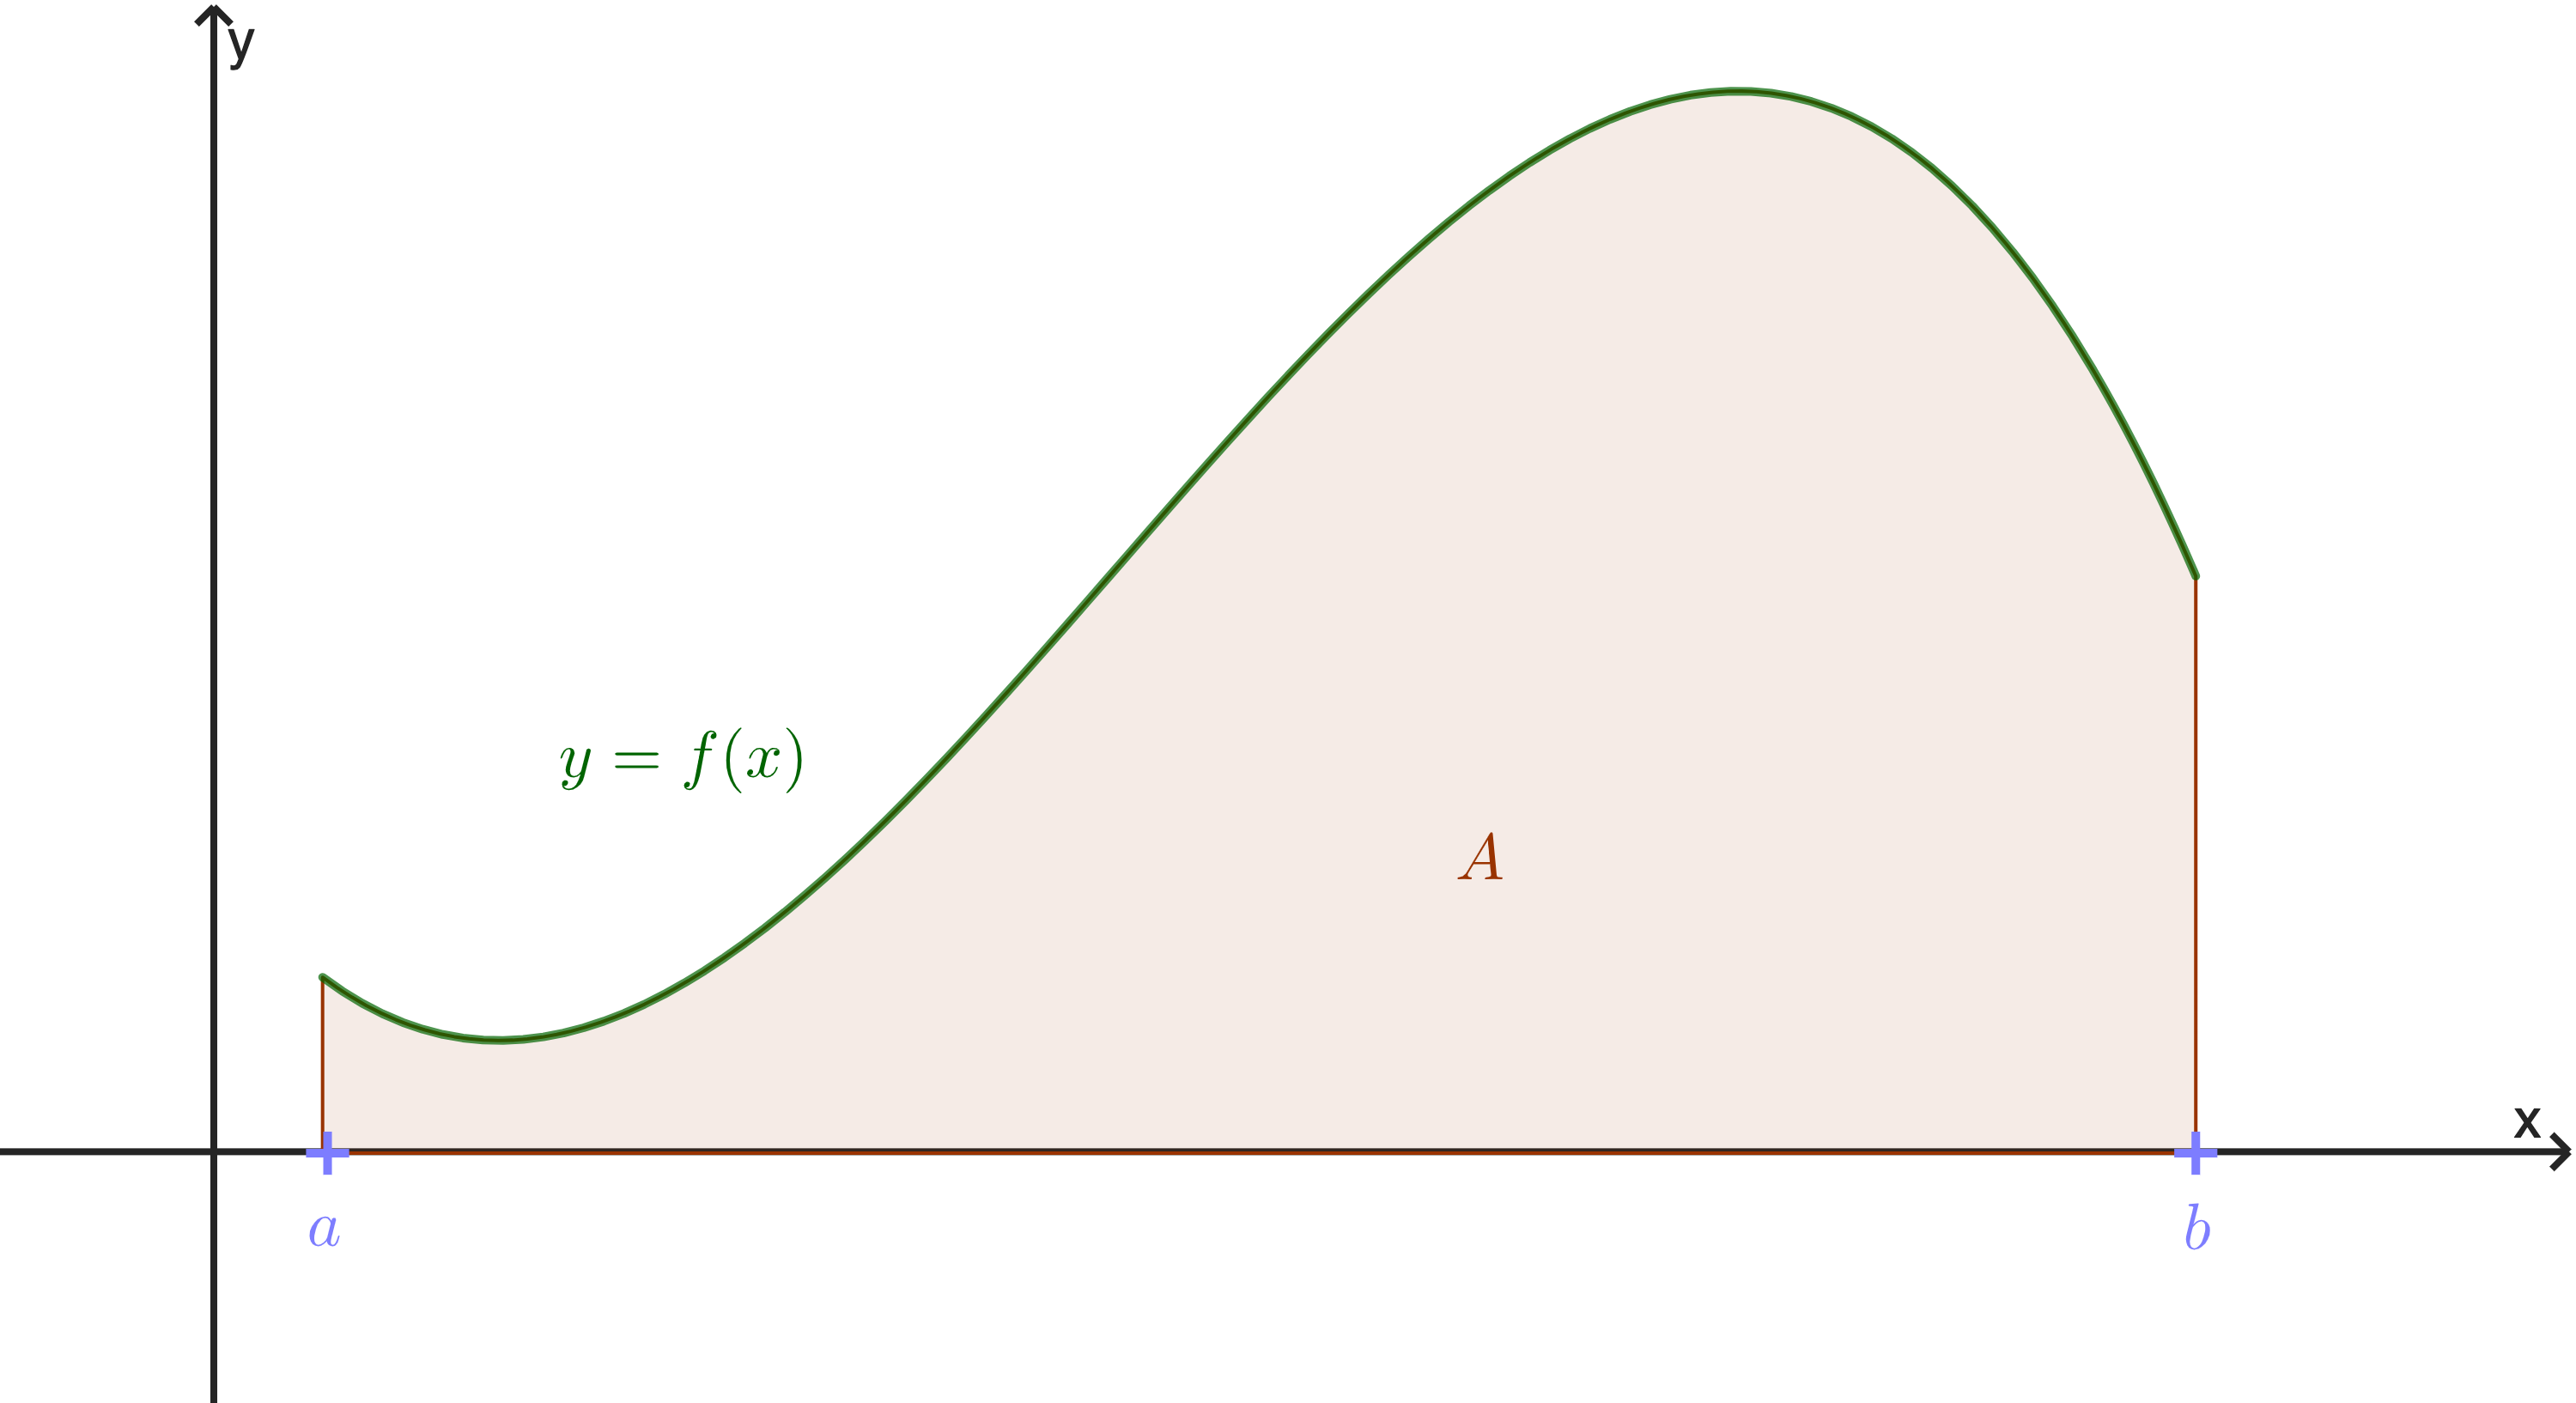
\includegraphics[width = 0.5\textwidth]{media/bestIntegral.png}
\end{center}
\clearpage
\begin{LA}{Einführungsaufgaben}{}
	Wenn die Funktion $f$ linear ist, können wir solche Flächeninhalte schon angeben.
	Berechnen Sie die schraffierten Flächeninhalte:
	\begin{enumerate}
		\item

		      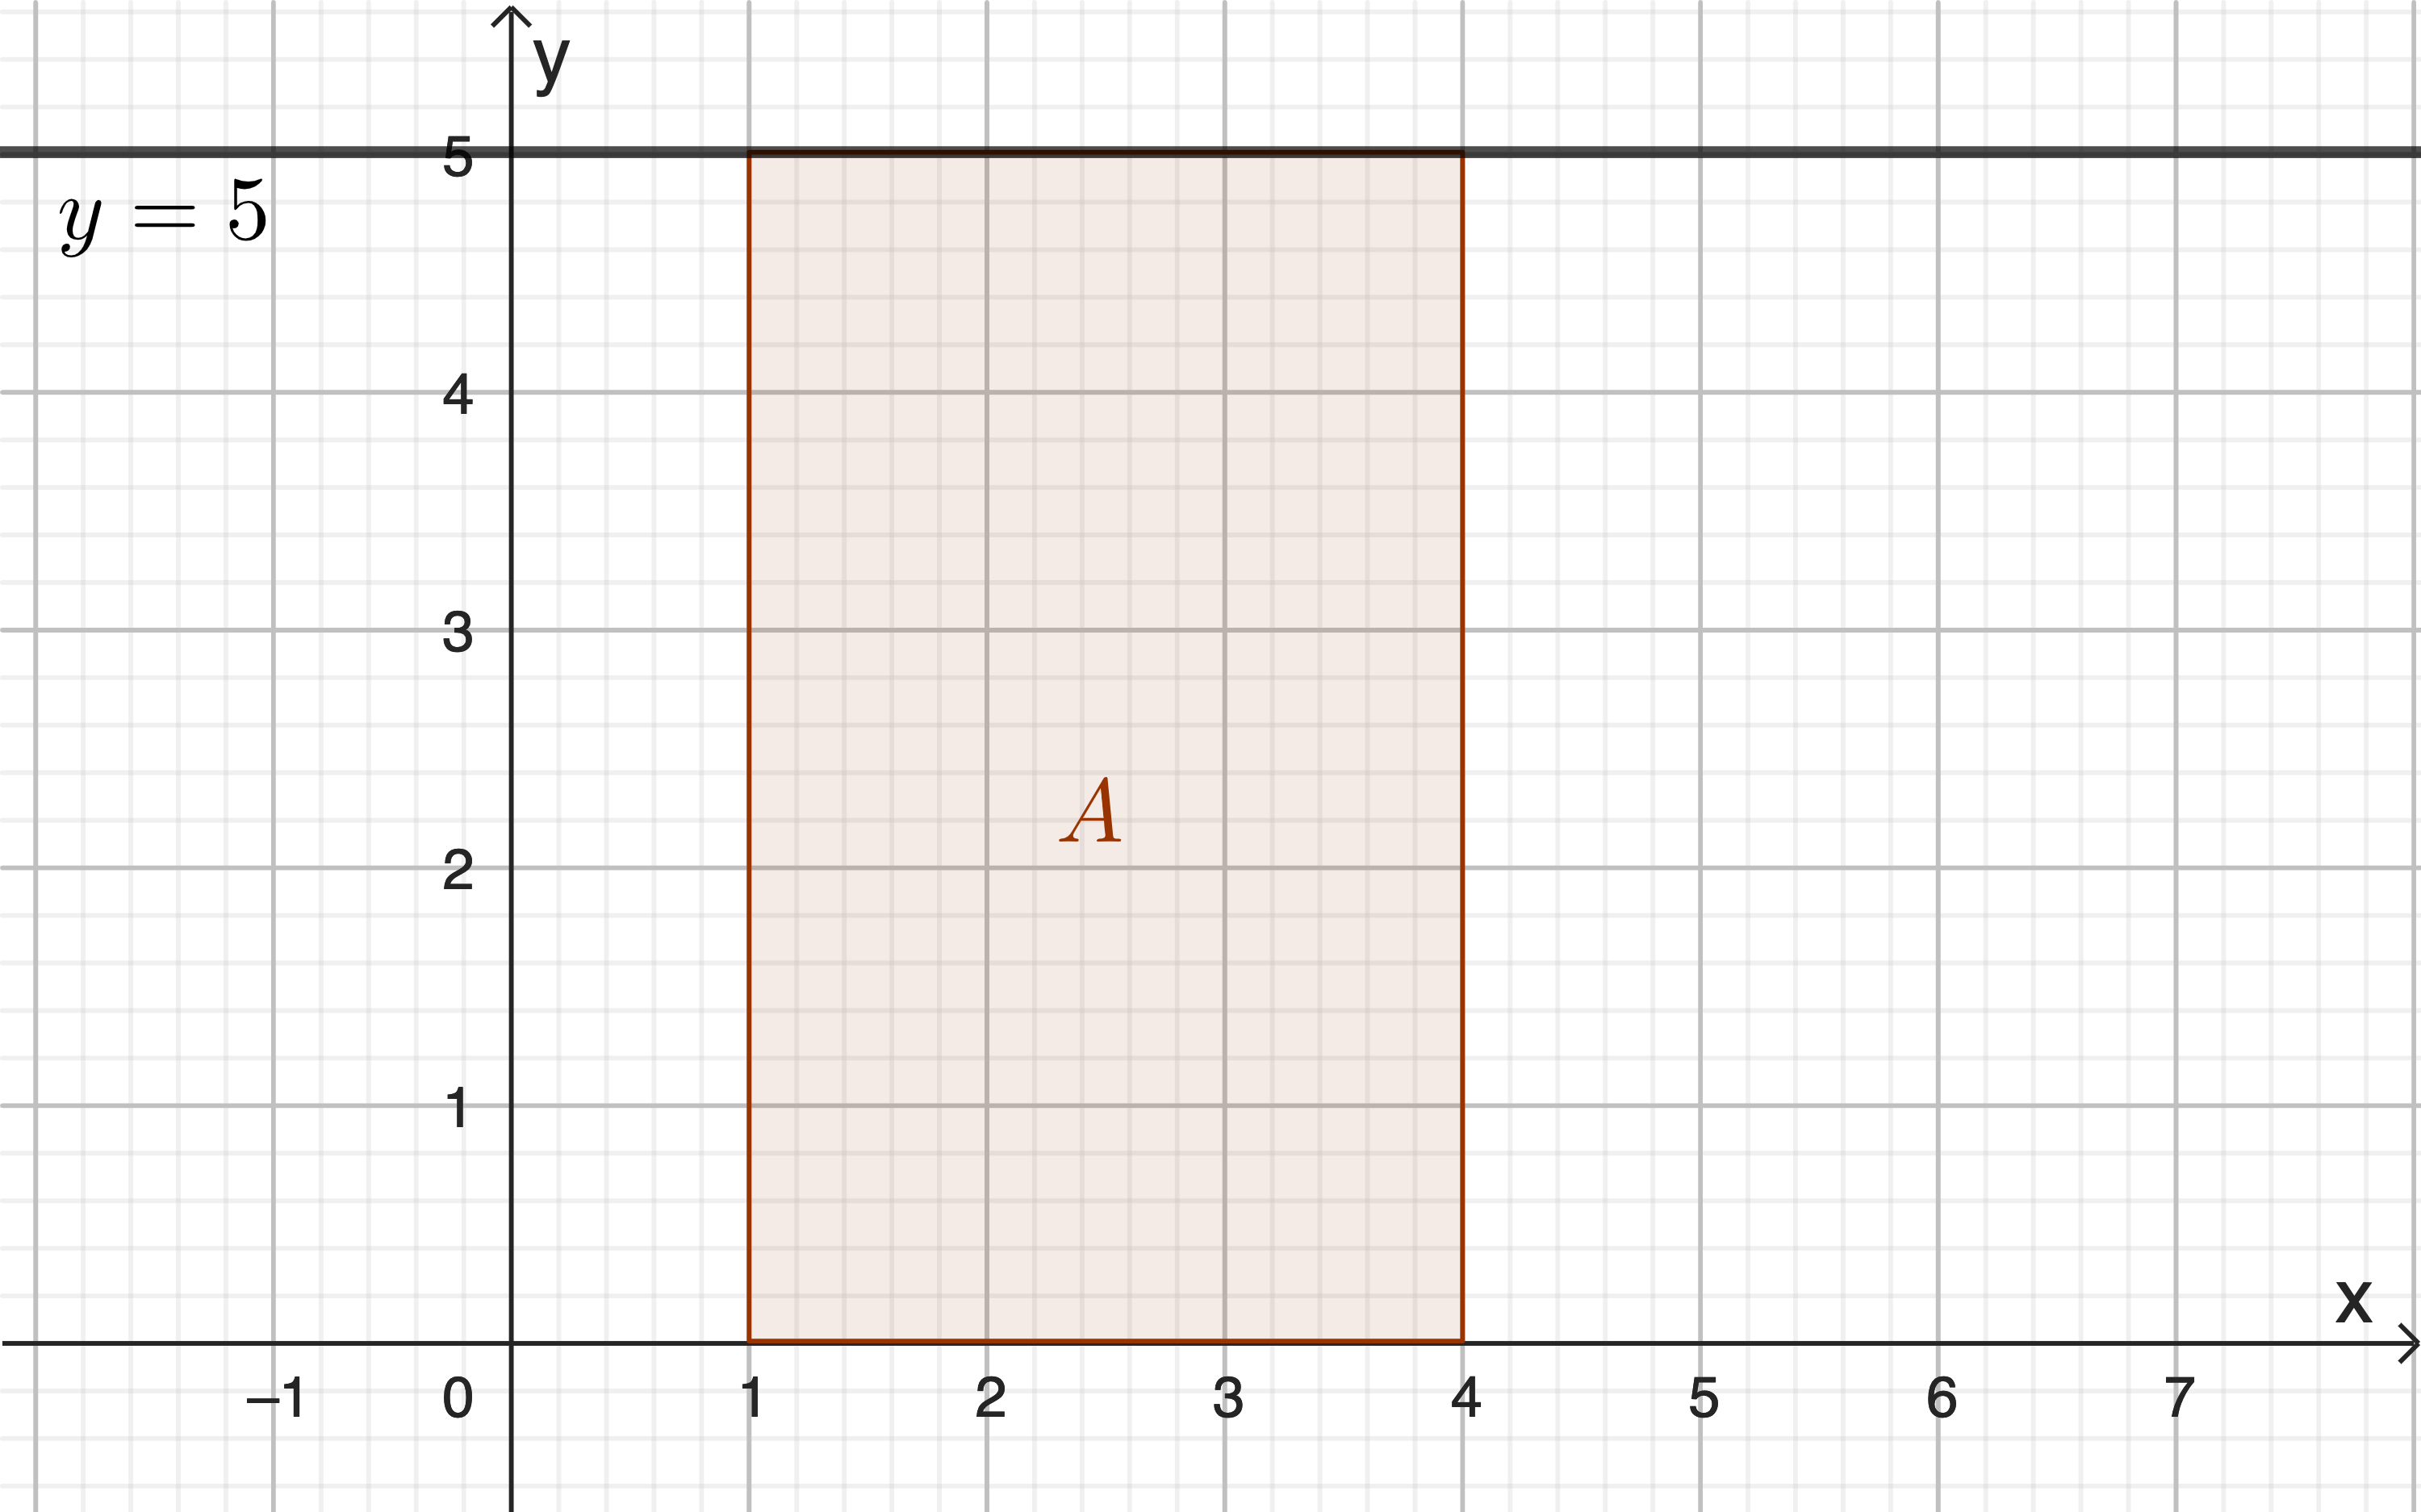
\includegraphics[width = 0.5\textwidth]{media/E-Bestimmt-Bsp1.png}
		\item

		      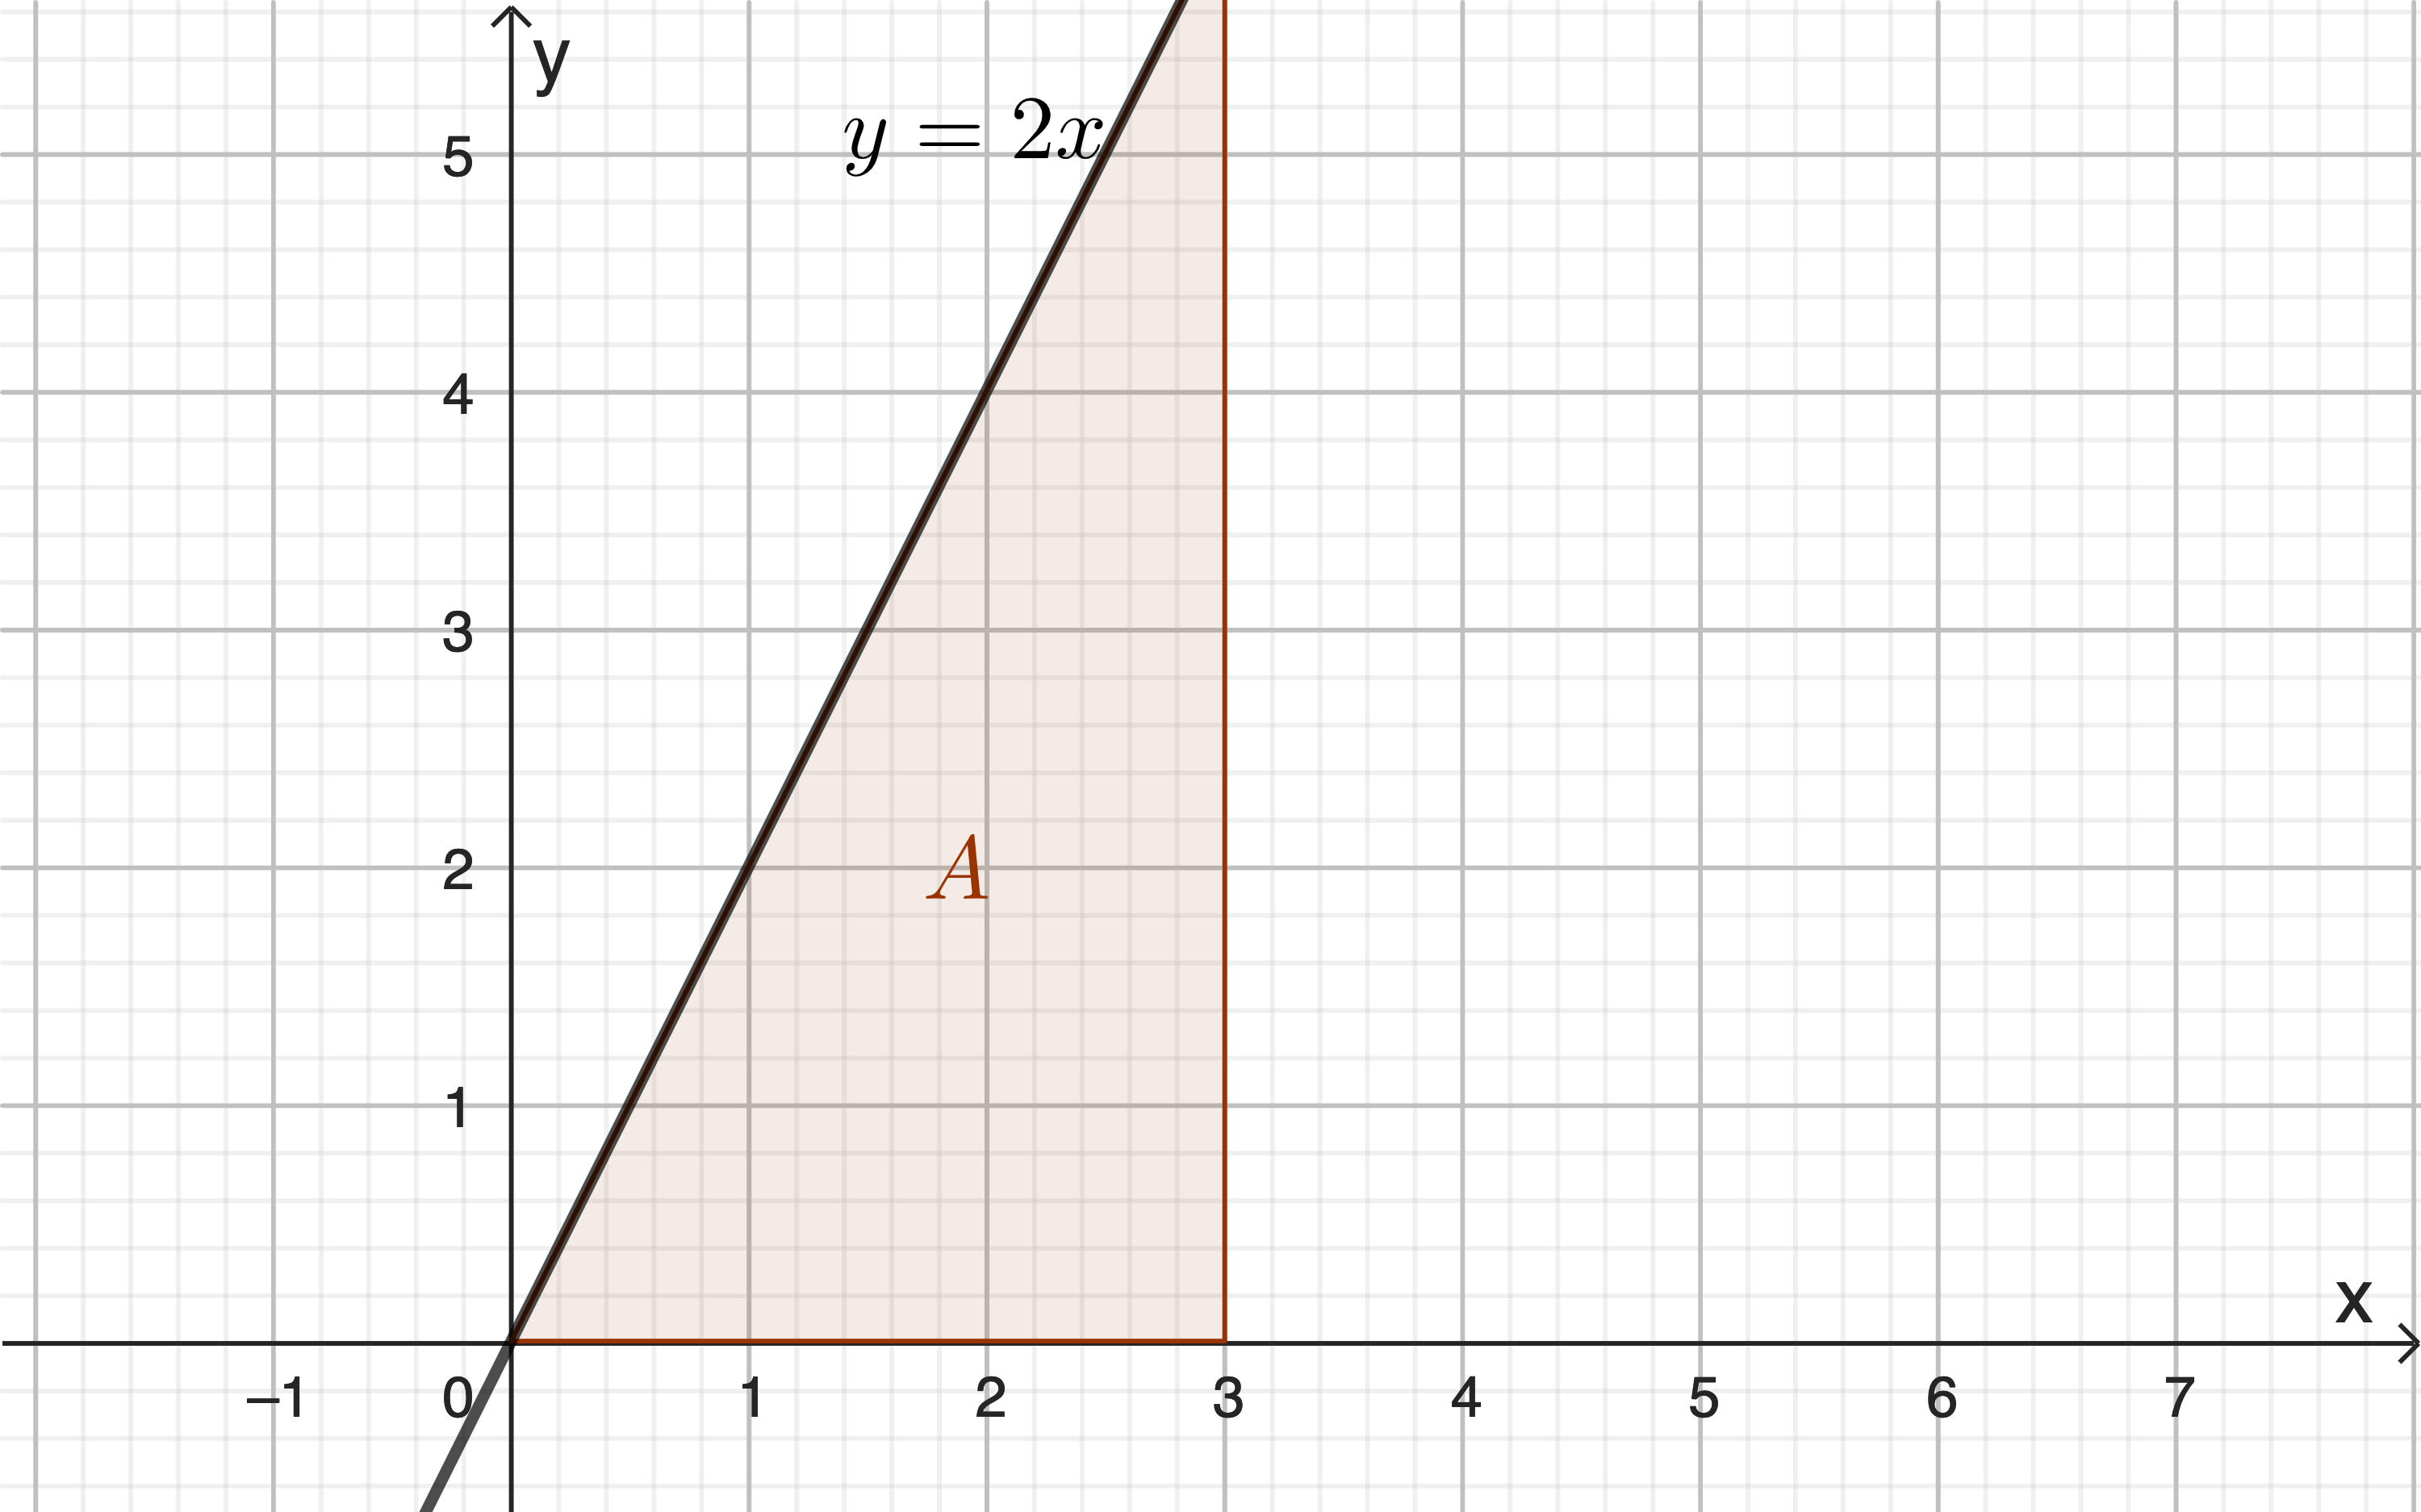
\includegraphics[width = 0.5\textwidth]{media/E-Bestimmt-Bsp2.png}
		\item

		      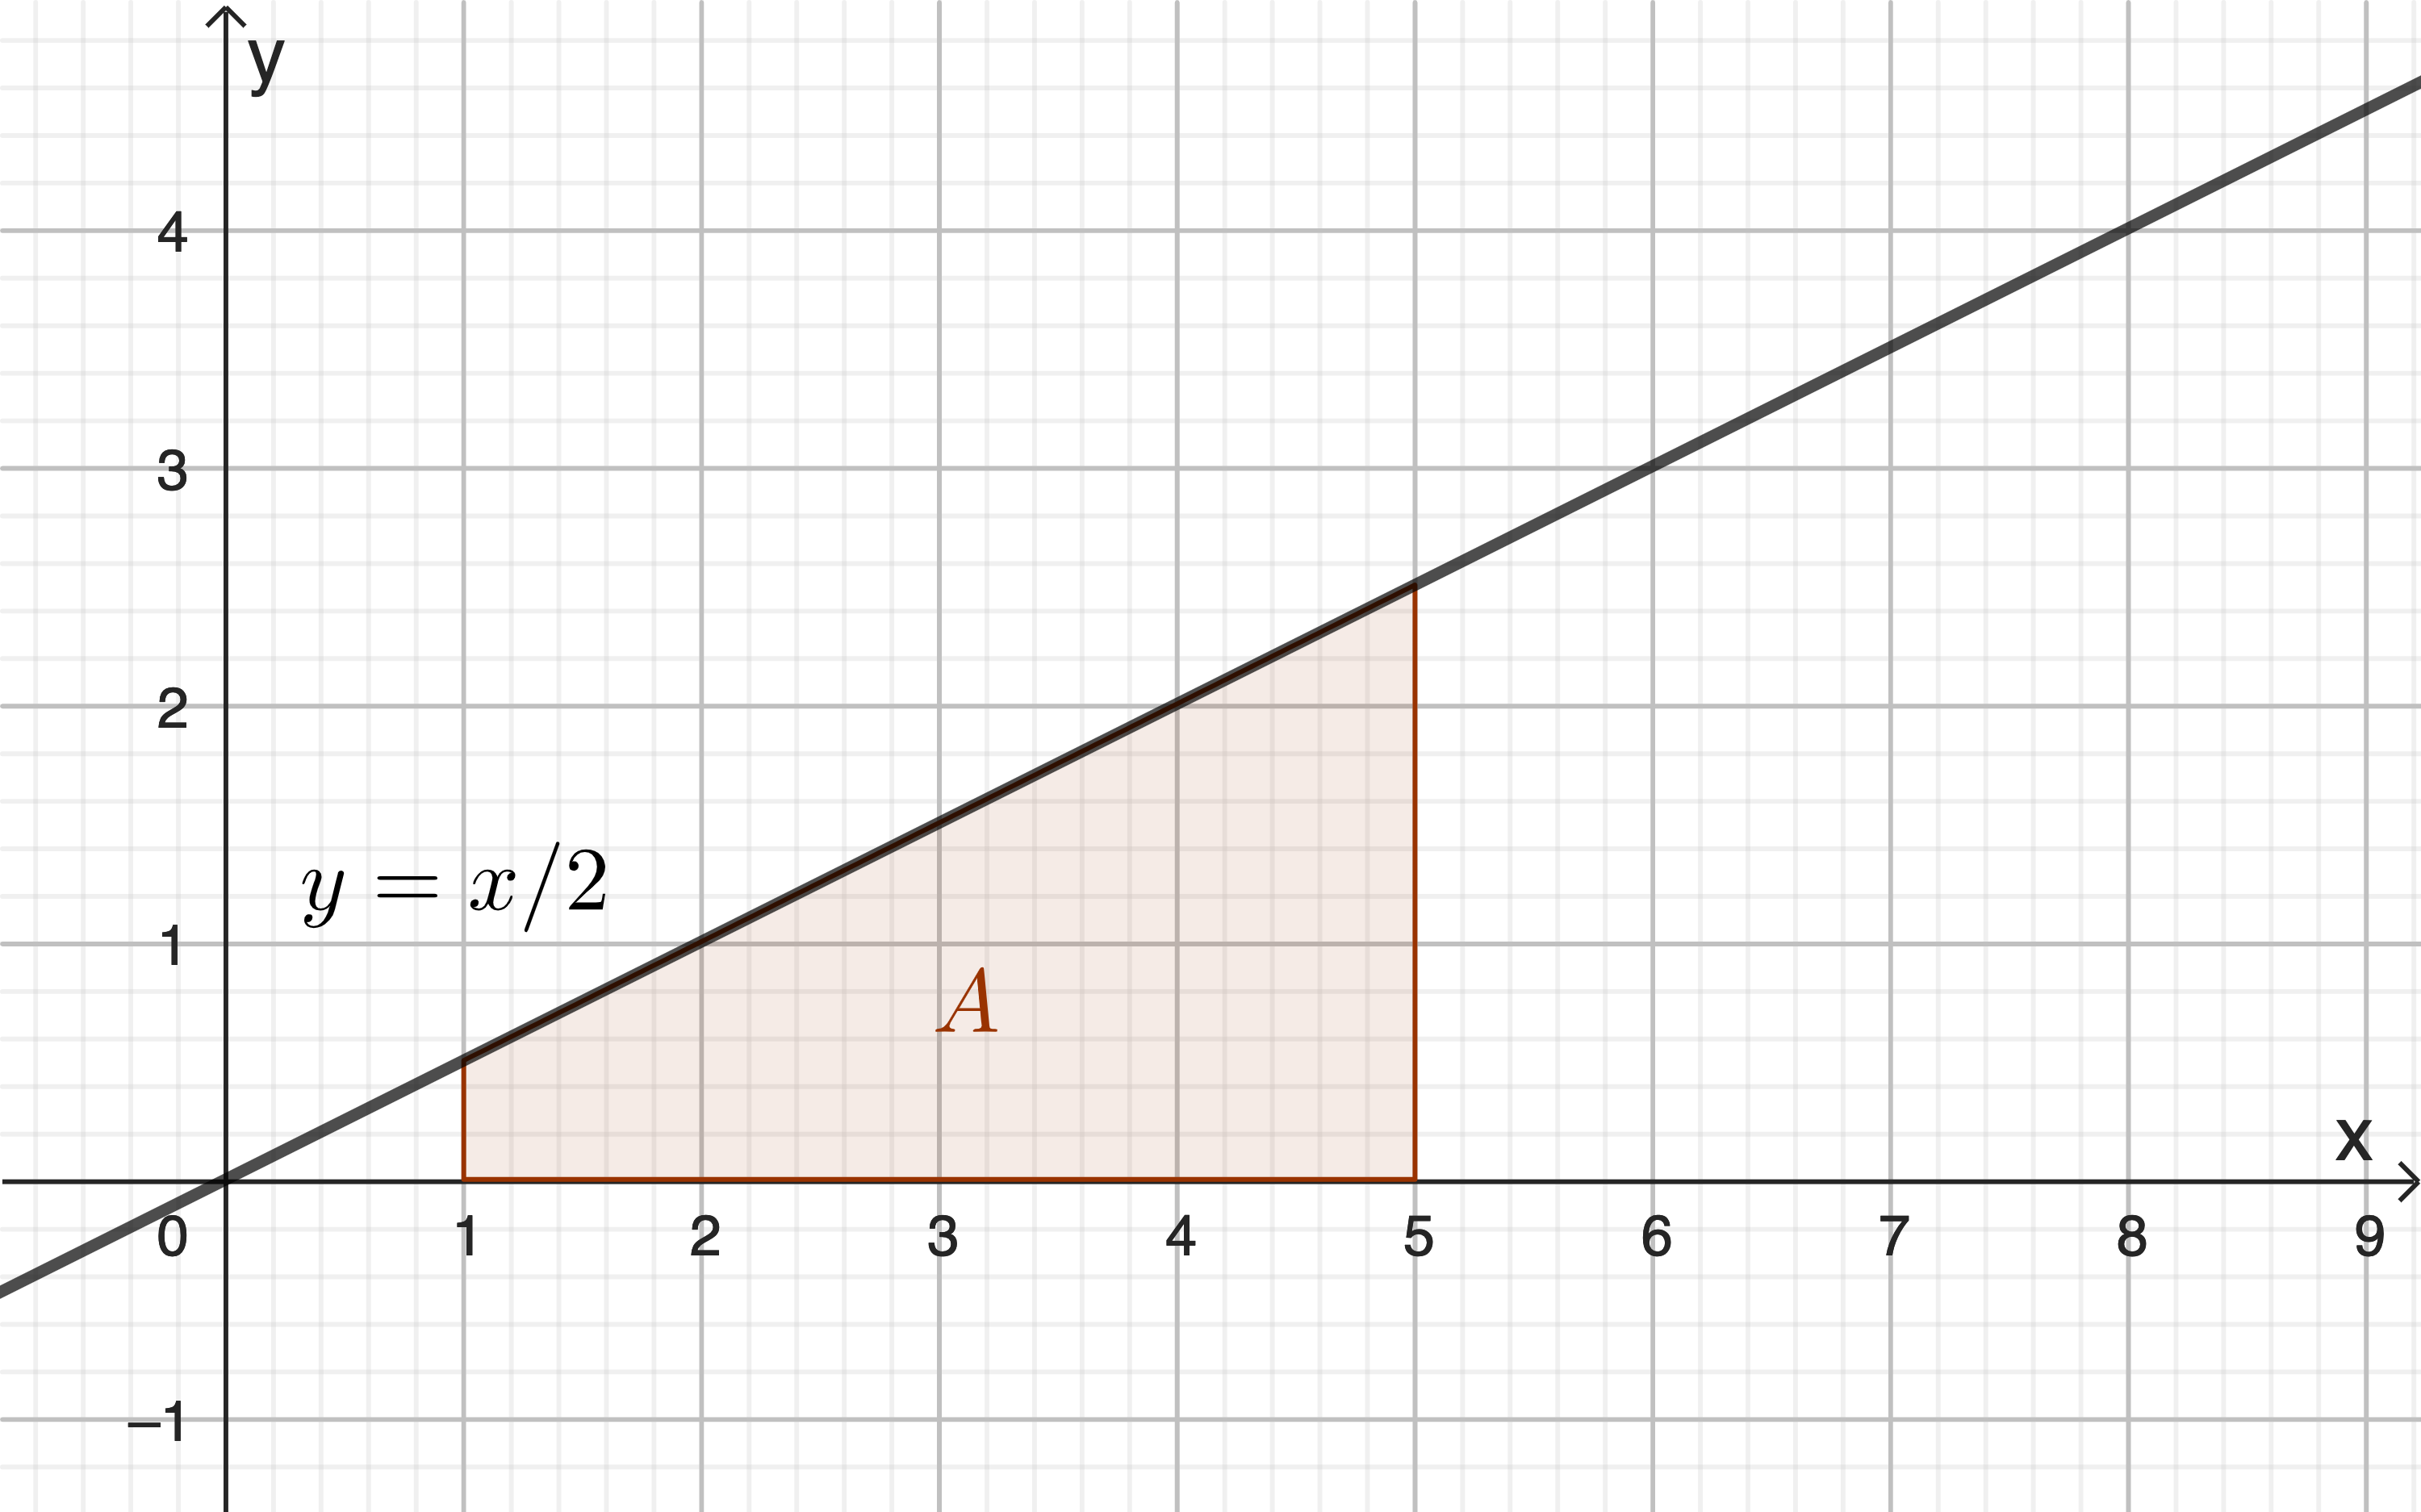
\includegraphics[width = 0.5\textwidth]{media/E-Bestimmt-Bsp3.png}
	\end{enumerate}

\end{LA}
\clearpage
Weil die Flächen in der Einführungsaufgabe durch geraden begrenzt sind, können die Flächeninhalte mit Hilfe von einfachen geometrischen Figuren berechnet werden. Anders sieht es aus, wenn die Fläche durch eine gekrümmte Linie begrenzt wird. Als Beispiel betrachten wir die Fläche unter dem Graphen der Funktion $f(x)=x^2$ im Intervall $[0, 1]$.

\begin{center}
	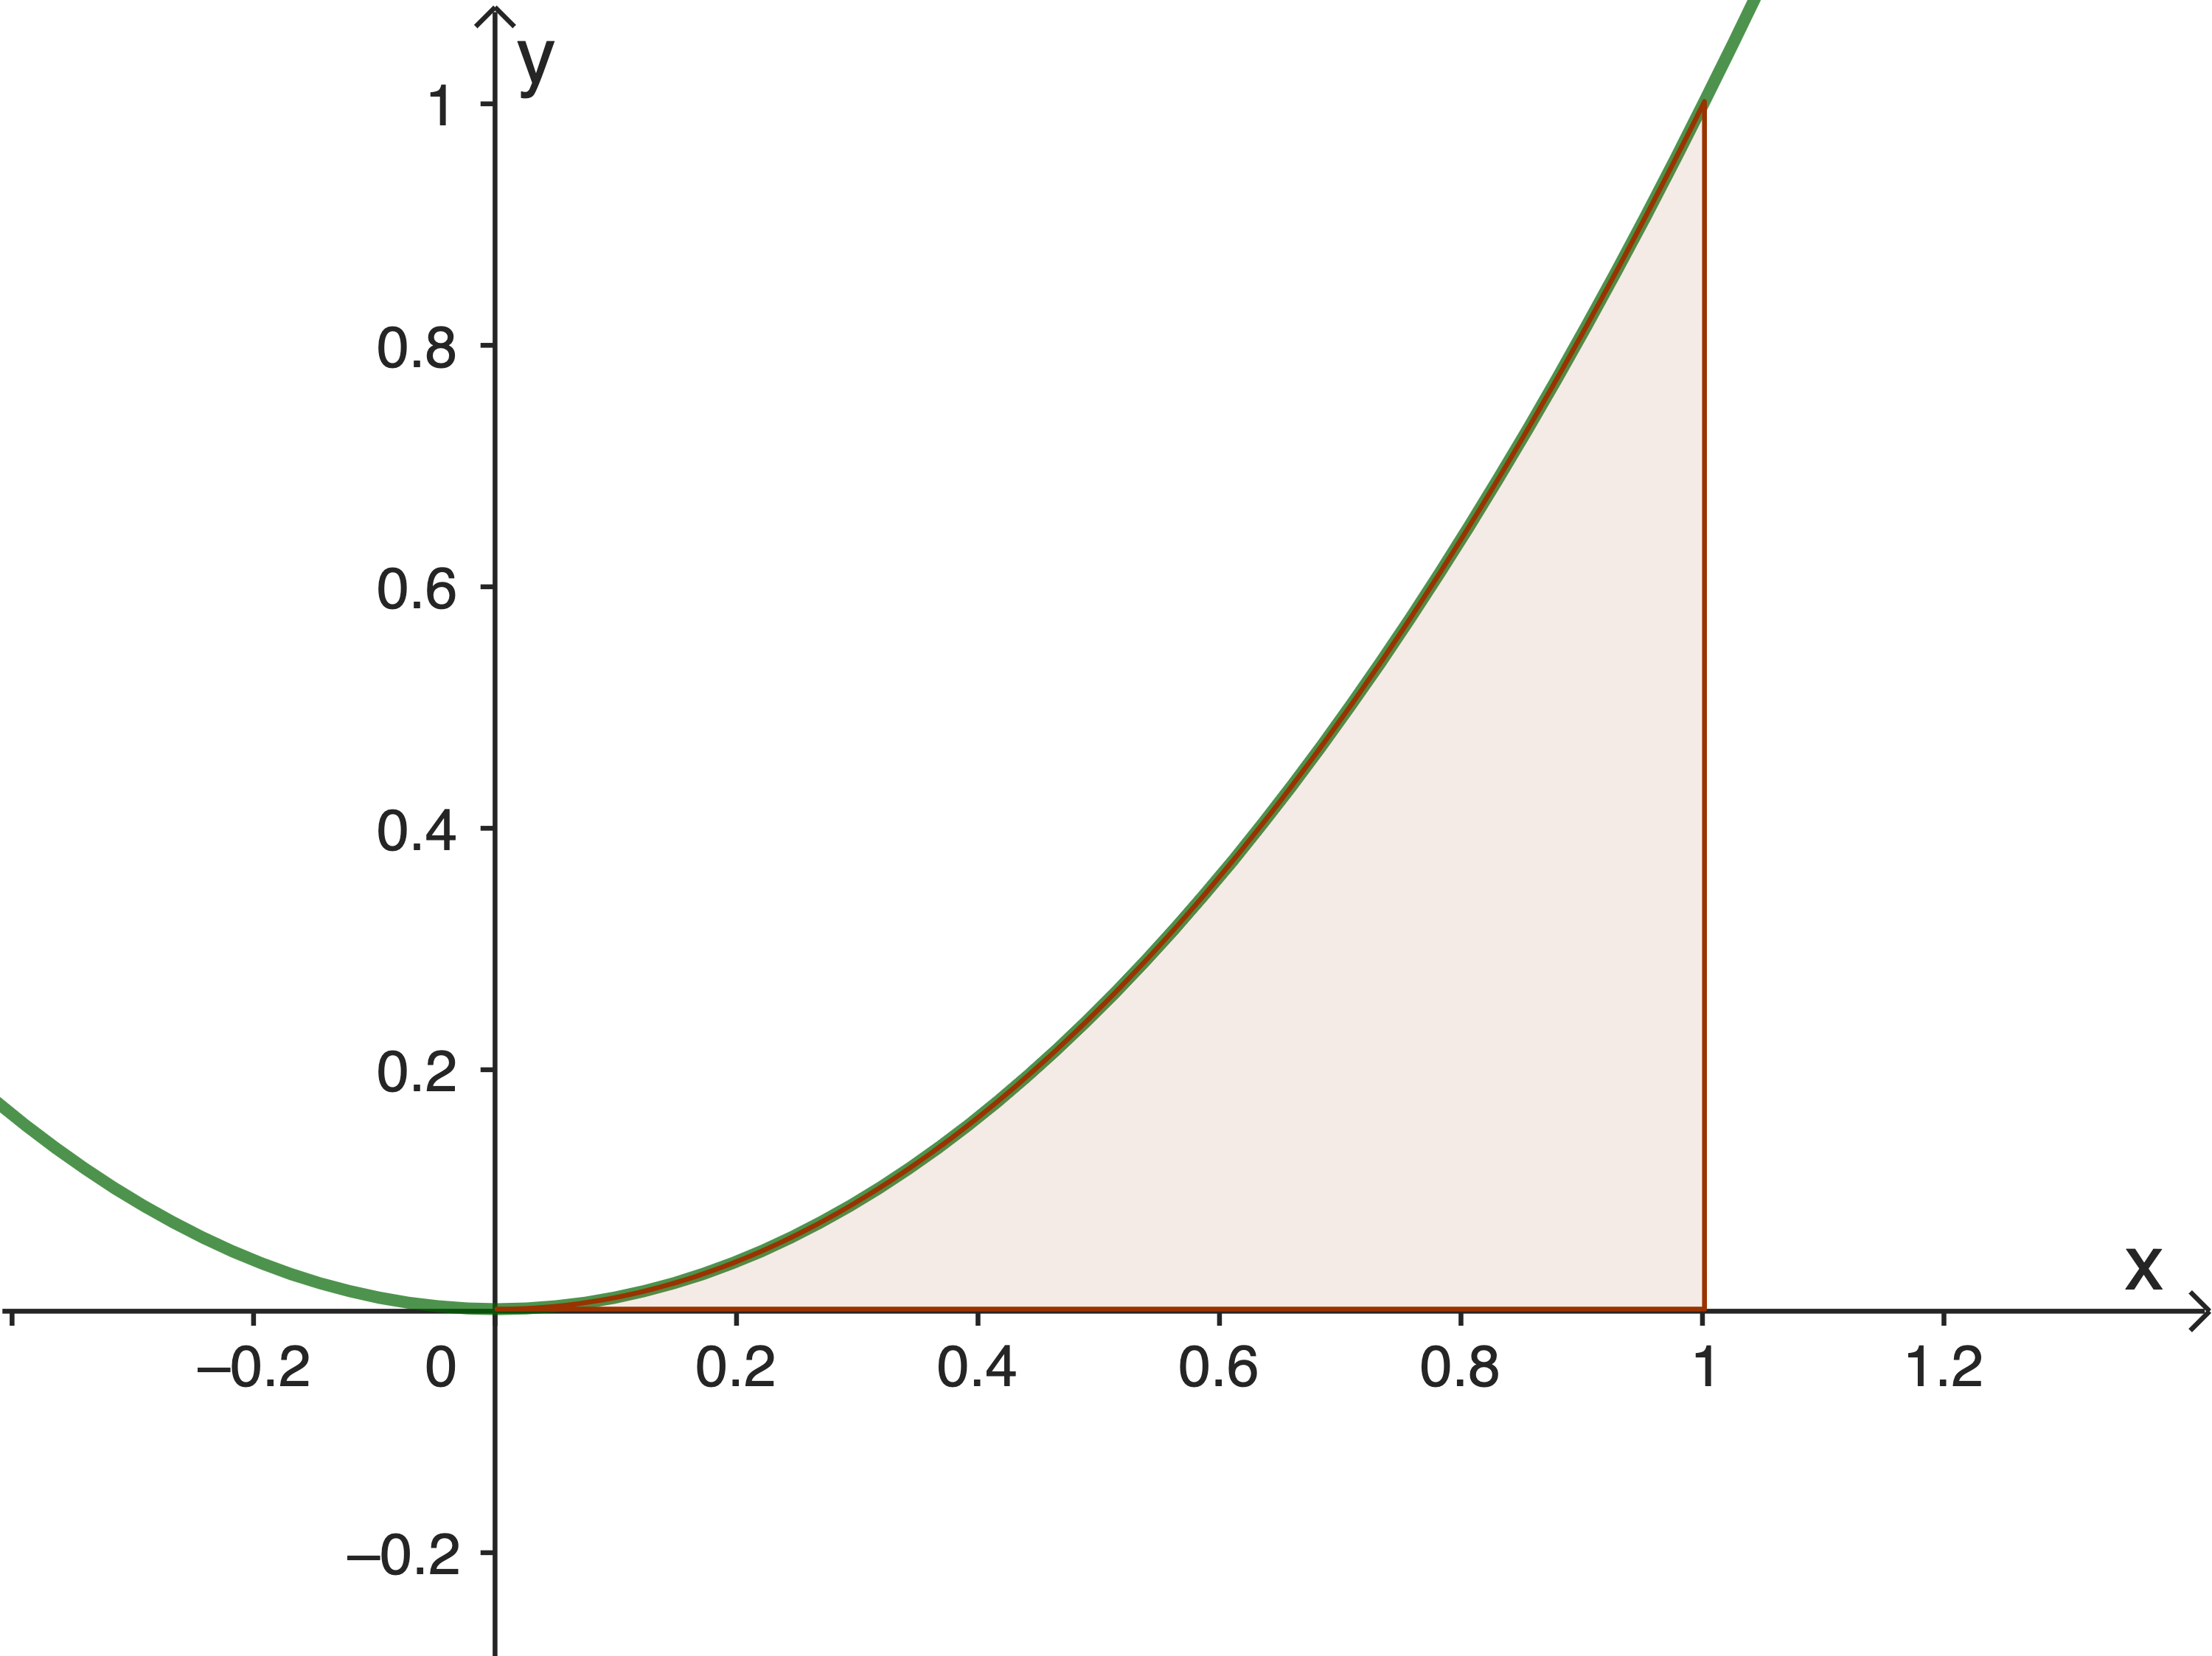
\includegraphics[width = 0.5\textwidth]{media/ober-untersumme-xquadrat.png}
\end{center}
Idee: Zur Bestimmung des Flächeninhalts unter der Parabel teilen wir das Intervall $[0,1]$ in vier Teile und betrachten zwei Näherungen für den Flächeninhalt.
\begin{center}
	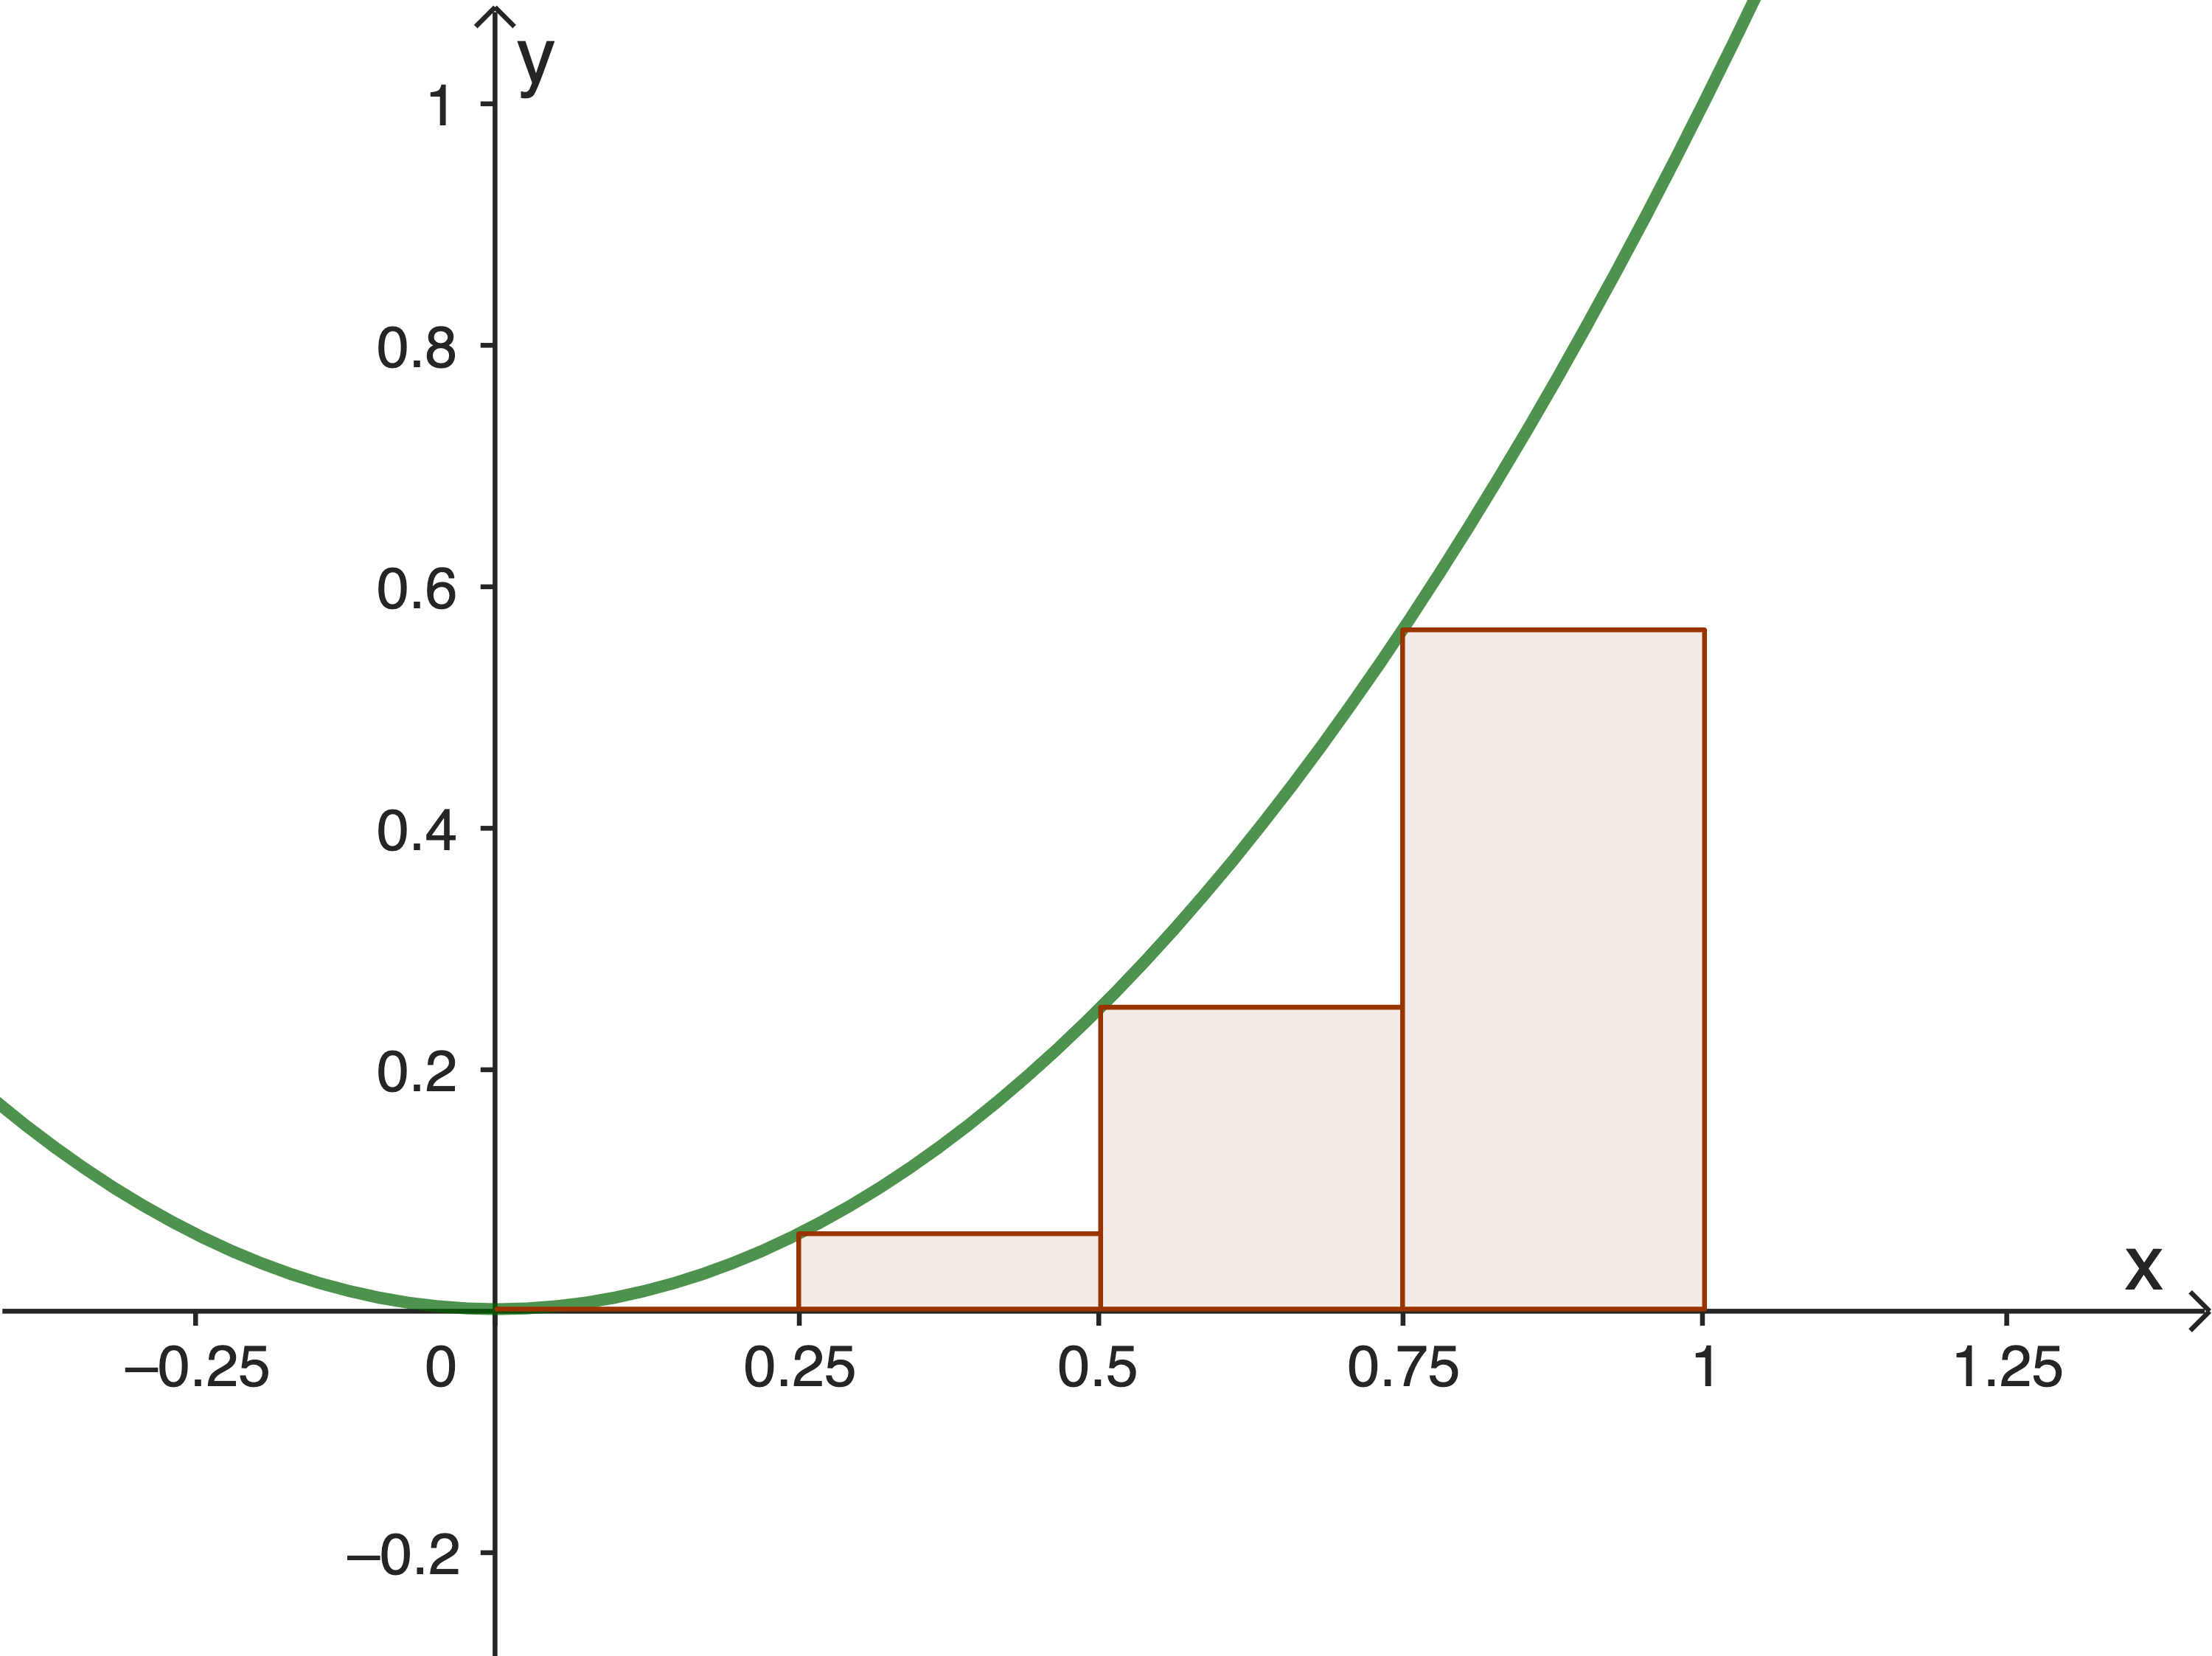
\includegraphics[width = 0.4\textwidth]{media/untersumme-x-quadrat.png}
	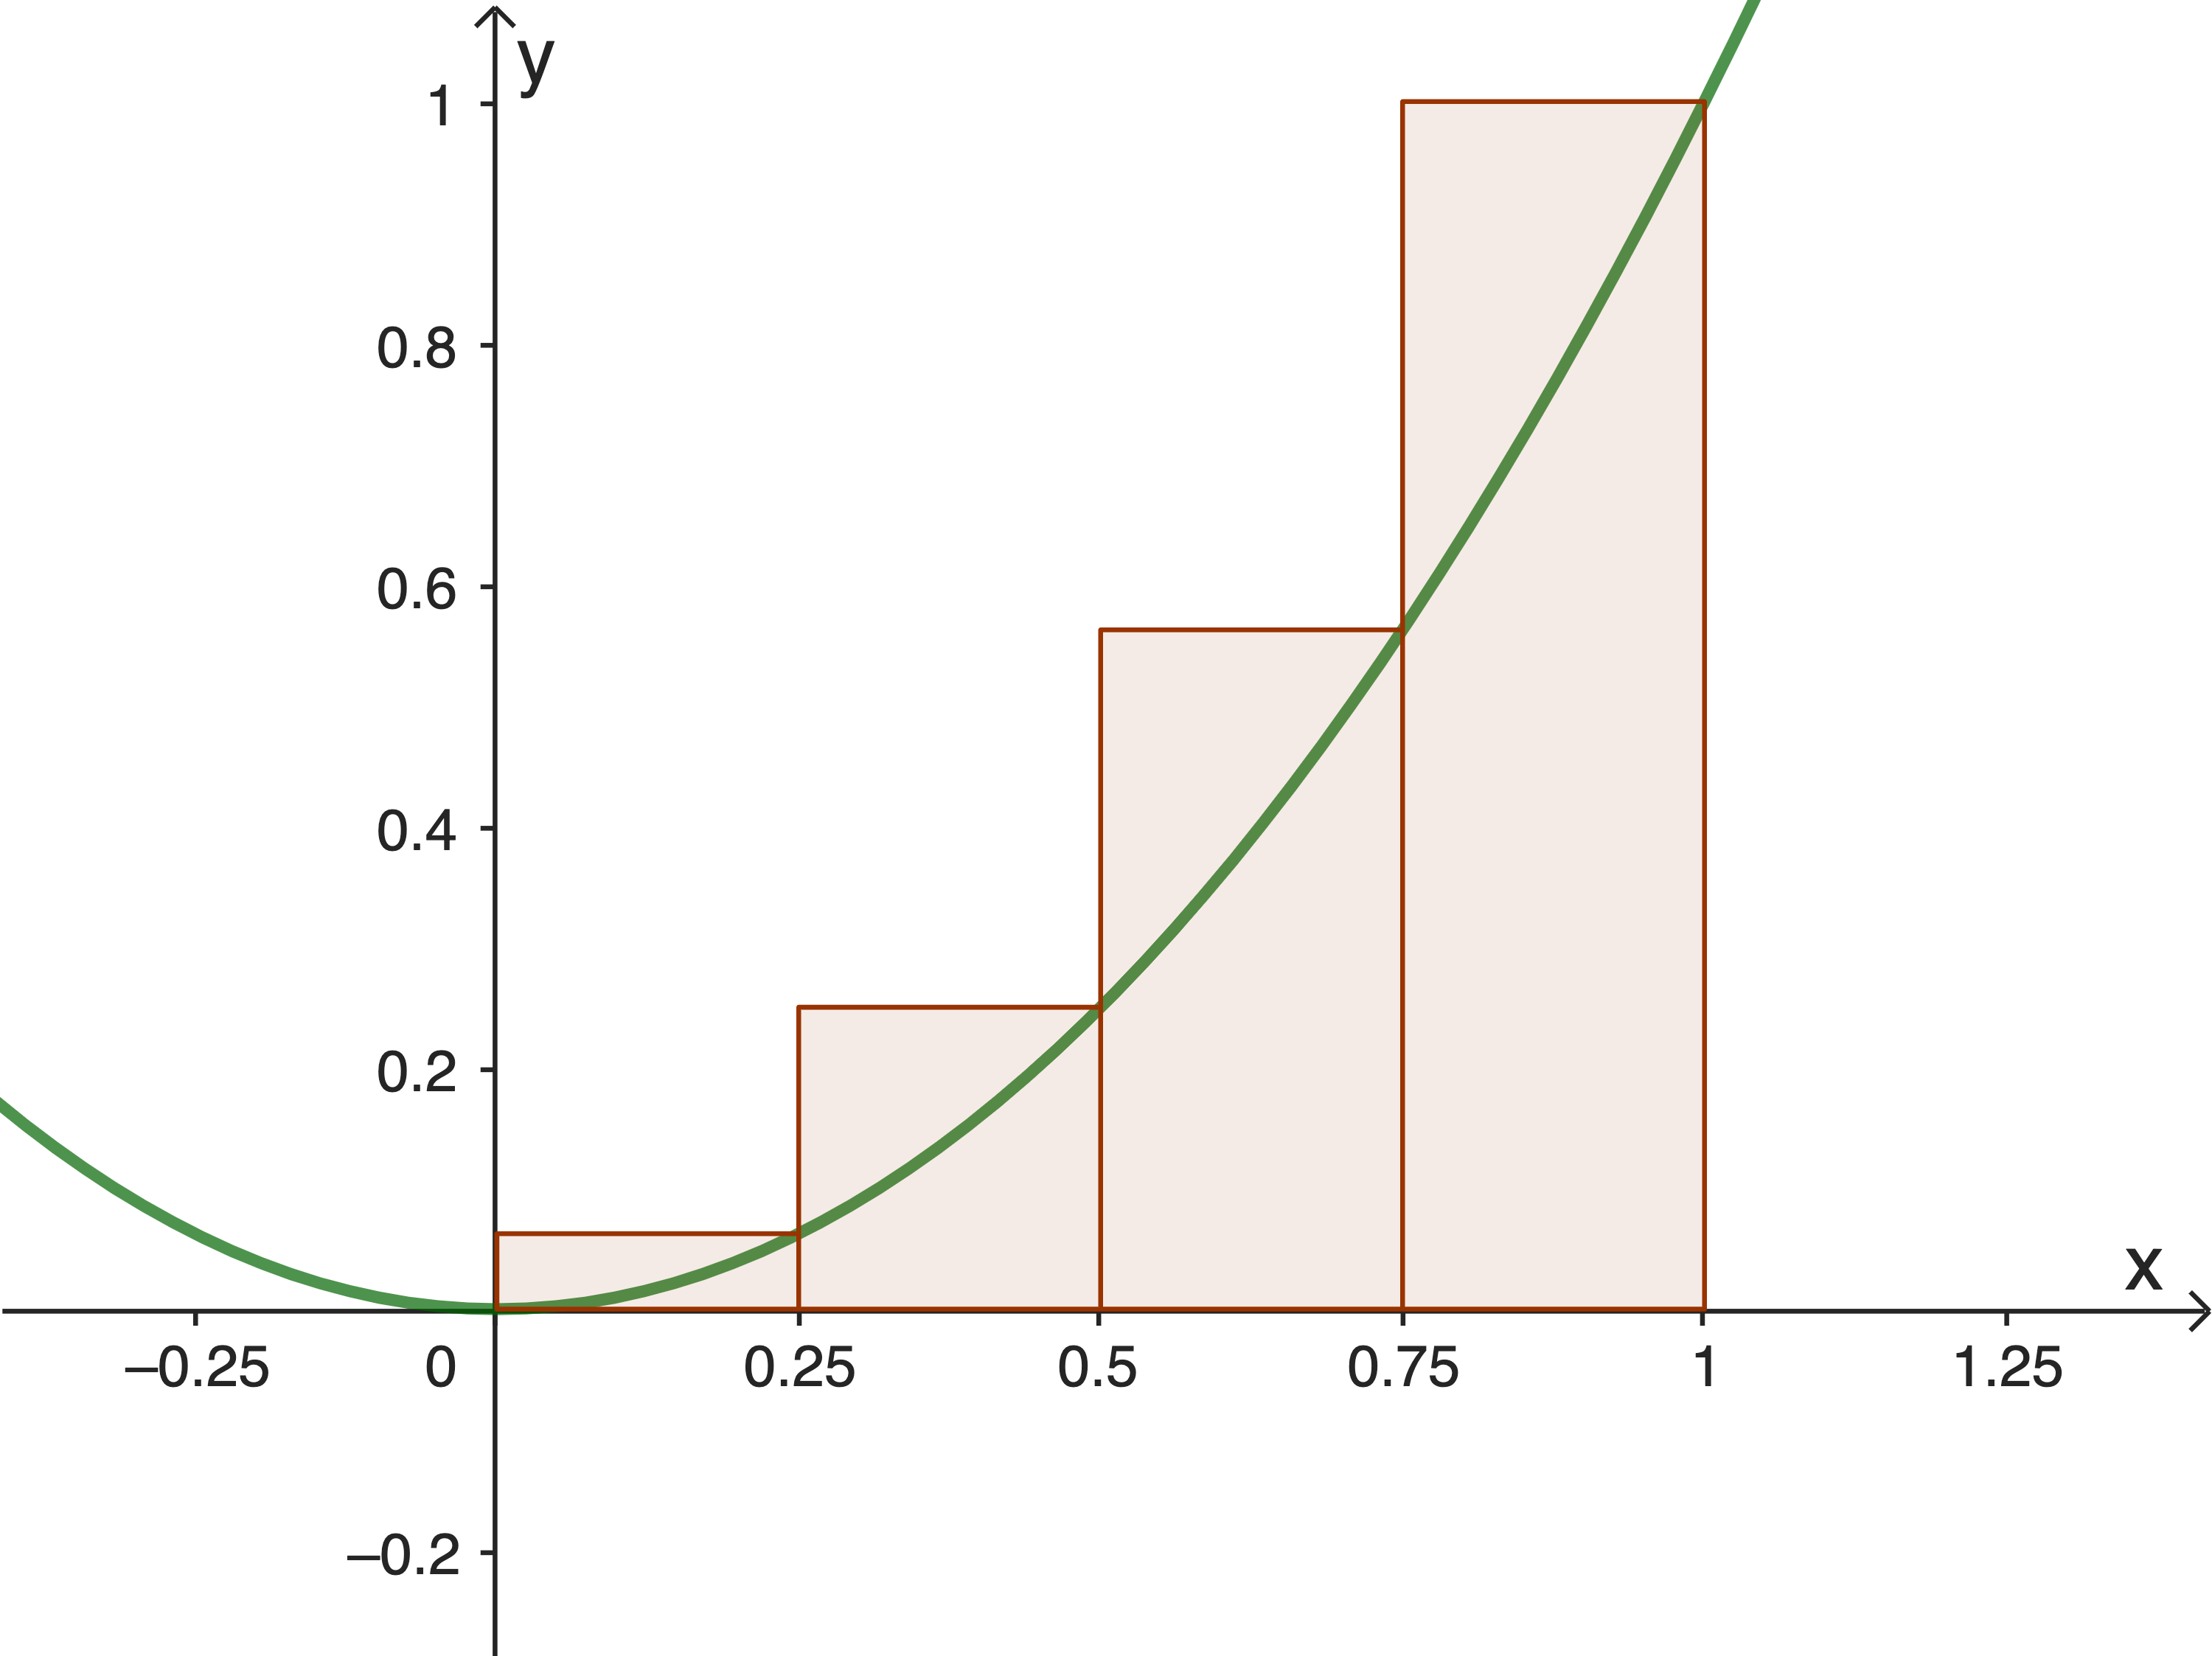
\includegraphics[width = 0.4\textwidth]{media/obersummex-quadrat.png}
\end{center}
Die Summe der Flächeninhalte der 4 Rechtecke in der Figur links nennen wir \textbf{Untersumme} $U_4$.(Beachten Sie, dass es ganz links ein \glqq Rechteck\grqq{} mit der Höhe 0 gibt). Die Summe der Flächeninhalte der 4 Rechtecke in der Figur rechts nennen wir \textbf{Obersumme} $O_4$. Der gesuchte Flächenihalt liegt also irgendwo zwischen $U_4$ und $O_4$. Je mehr Rechtecke wir verwenden, desto besser werden die Näherungen für den Flächeninhalt.

\clearpage
\begin{LA}
	{Die Fläche unter der Quadratfunktion - Teil 1}{FlächeUnterxQuadrat-teil1}
	\begin{enumerate}
		\item 	Zu den Figuren oben:
		      \begin{enumerate}
			      \item Berechnen Sie die beiden Näherungen $U_4$ und $O_4$. \\
			            (Kontrolle: $U_4=\frac{7}{32}$ und $O_4=\frac{15}{32} $)
			      \item Wird das Intervall $[0,1]$ in $8$ Teile zerlegt, erhält man bessere Approximationen (= Näherungen) für den Inhalt der Fläche unter der Parabel. Berechnen Sie $U_8$ und $O_8$.
			            (Kontrolle: $U_8=\frac{35}{128}; \; O_8=\frac{51}{128}$ )
		      \end{enumerate}
		\item Challenges:
		      \begin{enumerate}
			      \item 	Bestimmen Sie je einen Term für die Unter- bzw. Obersumme, wenn man das Intervall in $n$ Teile unterteilt.
			      \item 	Für jedes Zahl $k\in \N$ gilt
			            $$ 1+4+9+16+ \cdots +k^2=\frac{k(k+1)(2k+1)}{6}.$$
			            Verwenden Sie diese Formel, um die Ober- und Untersumme weiter zu vereinfachen.
			      \item Welchen Grenzwert erhält man für die beiden Summen, für $n \rightarrow \infty$?.
		      \end{enumerate}

	\end{enumerate}
\end{LA}

\clearpage

Mit dem Grenzwert von Ober- und Untersumme haben wir eine Methode gefunden, mit der man den Flächeninhalt von beliebigen Gebieten unter der Quadratfunktion berechnen kann.

\begin{center}
	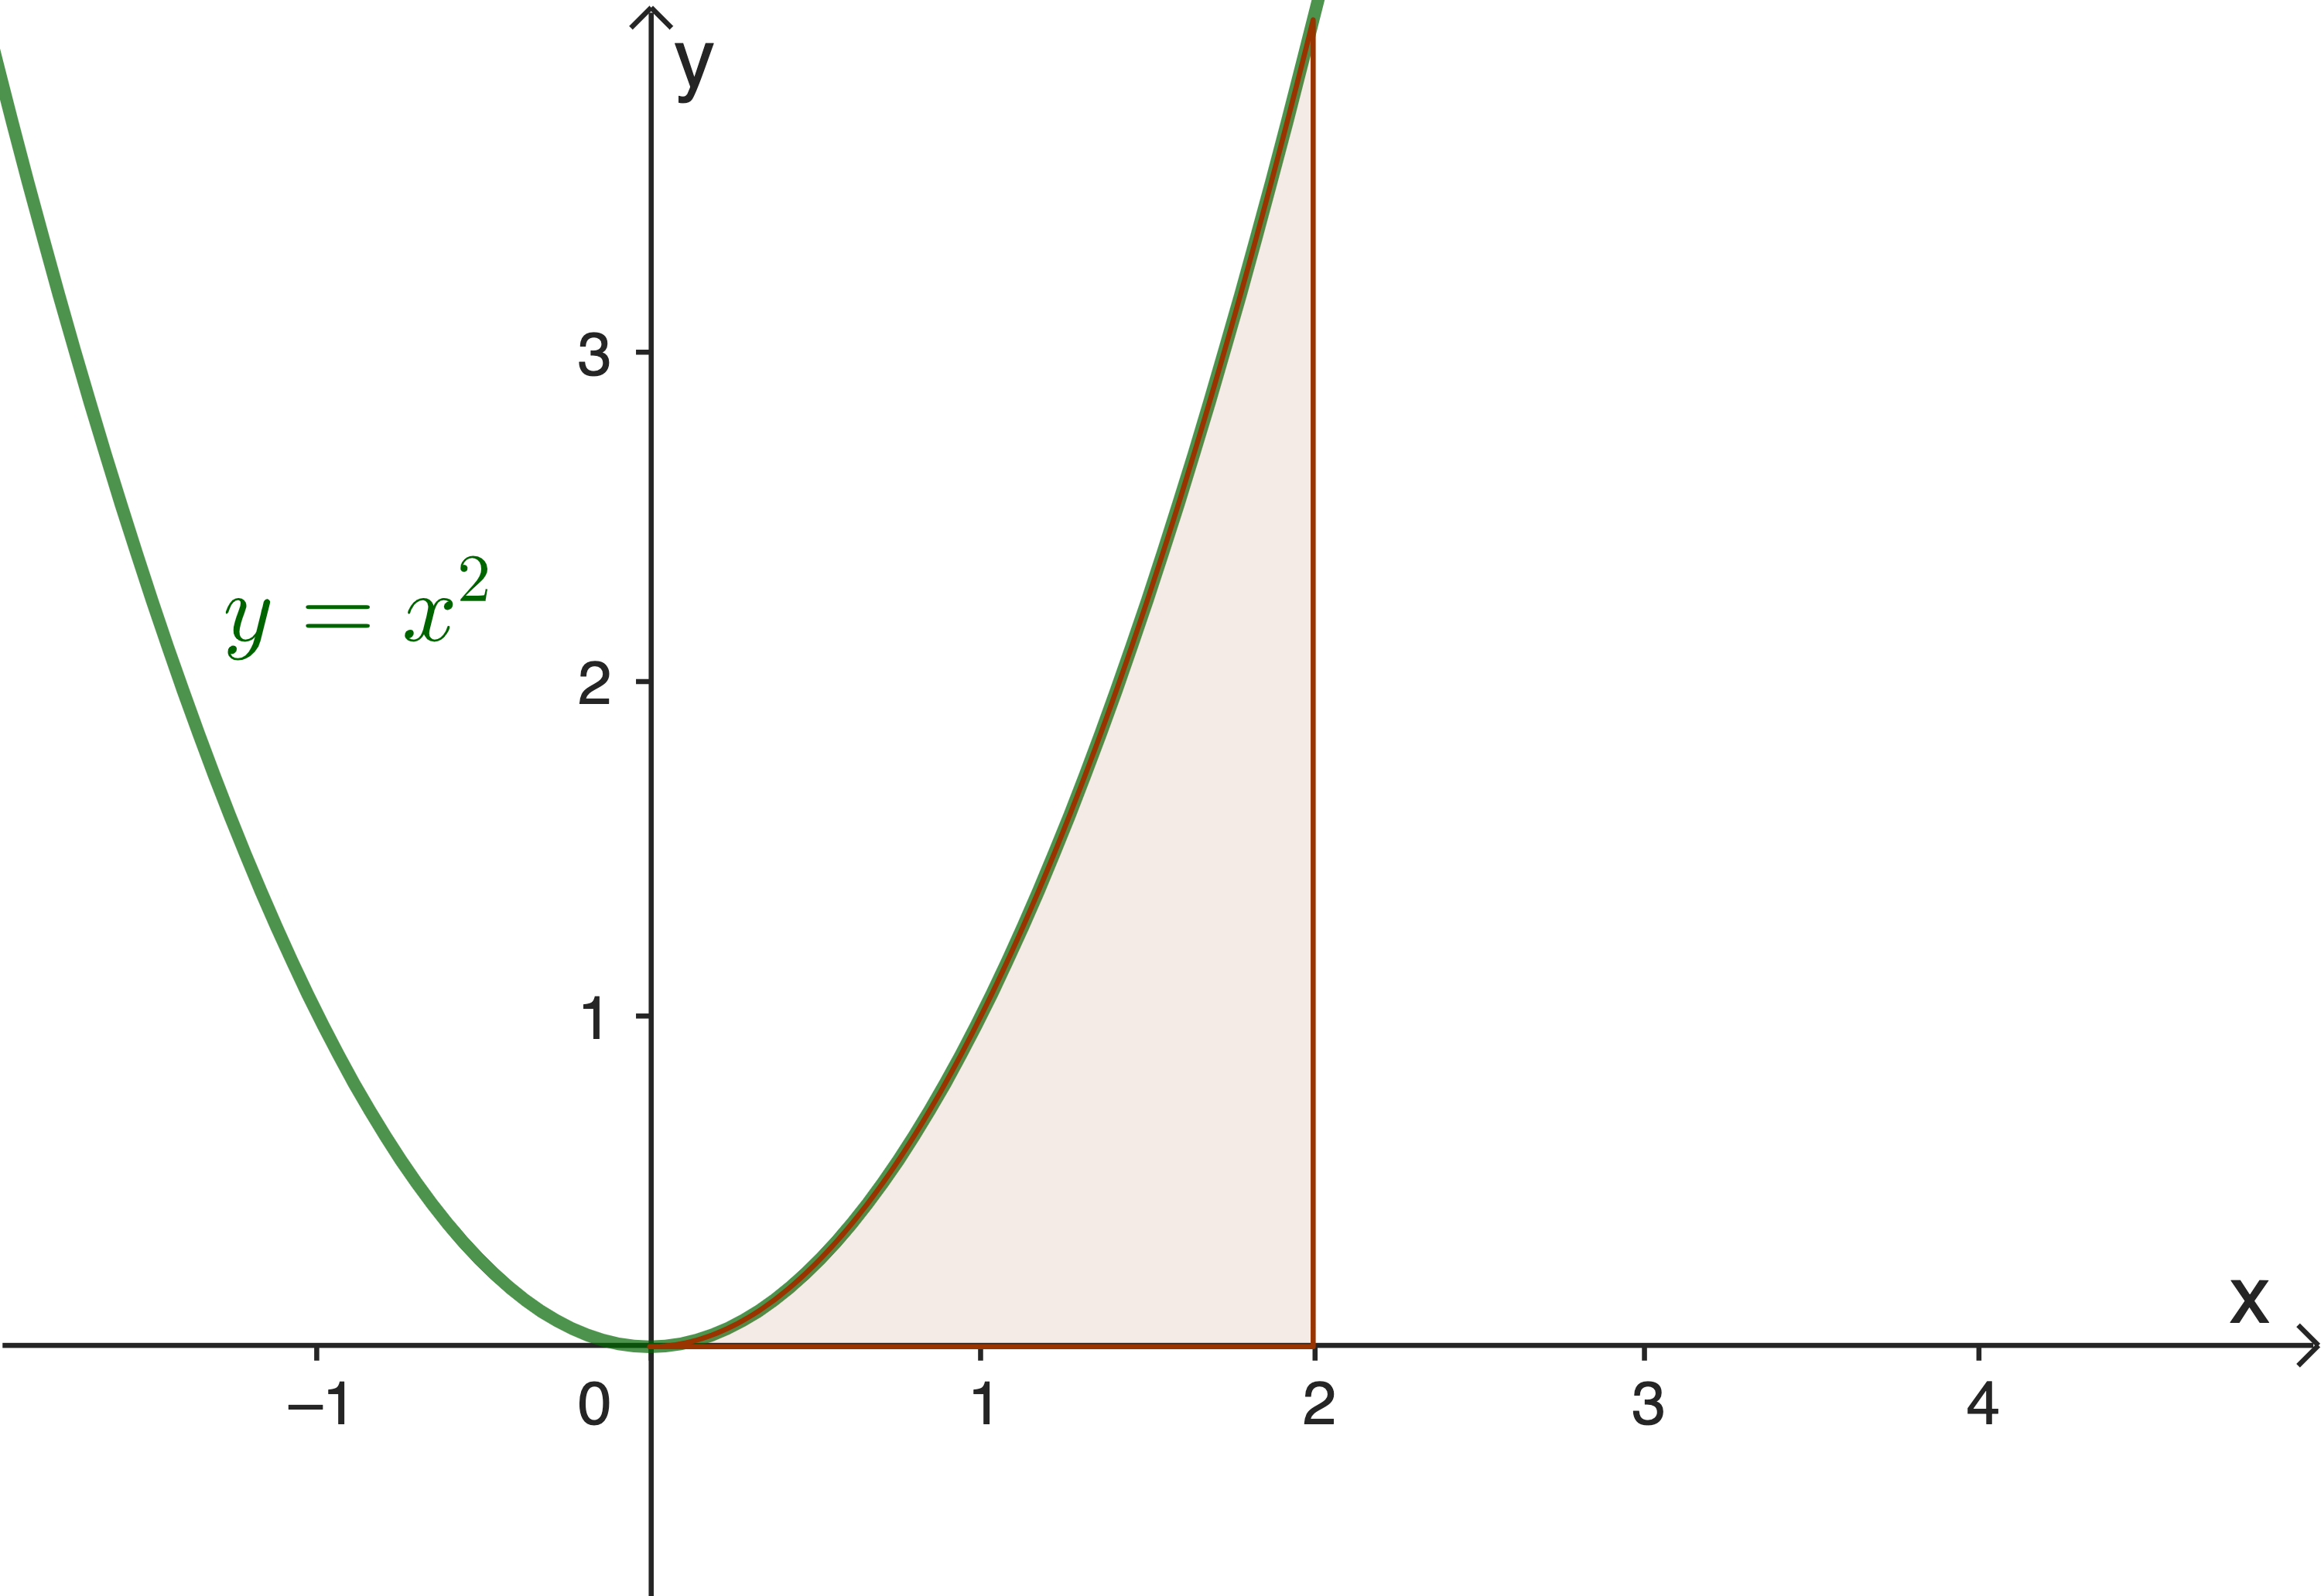
\includegraphics[width = 0.25\textwidth]{media/integral0-2-xquadrat.png}
	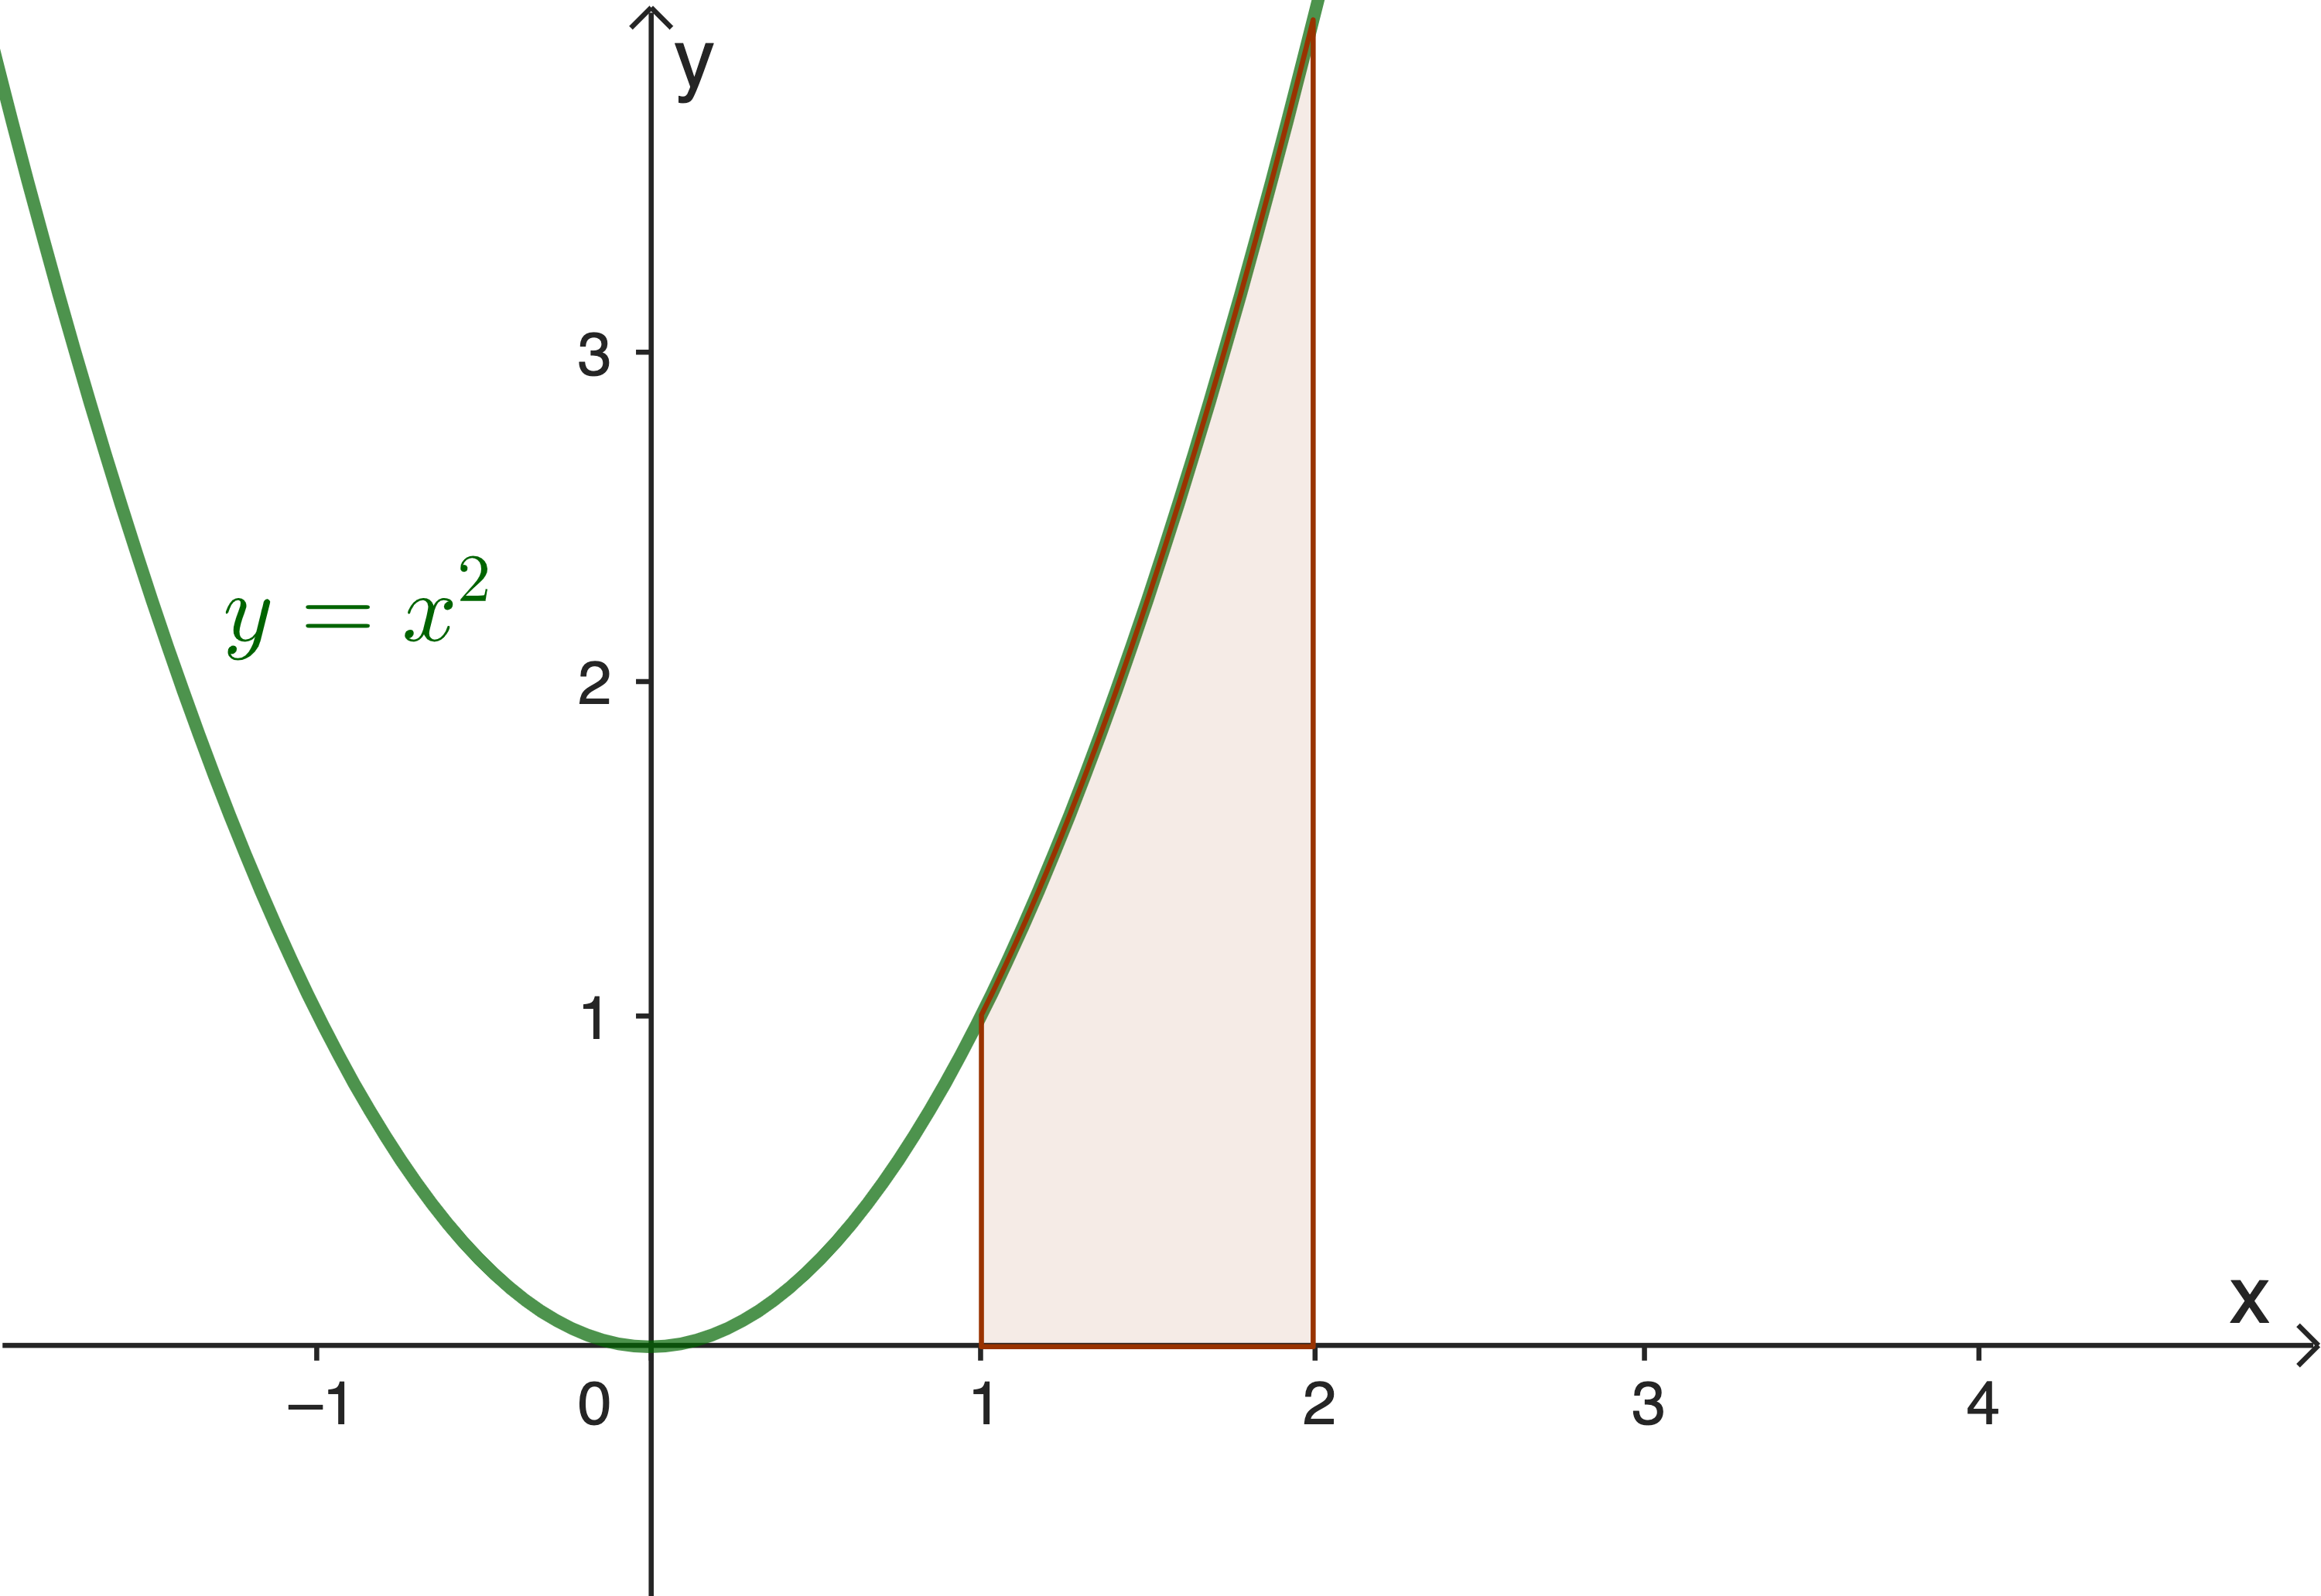
\includegraphics[width = 0.25\textwidth]{media/integral1-2-xquadrat.png}
	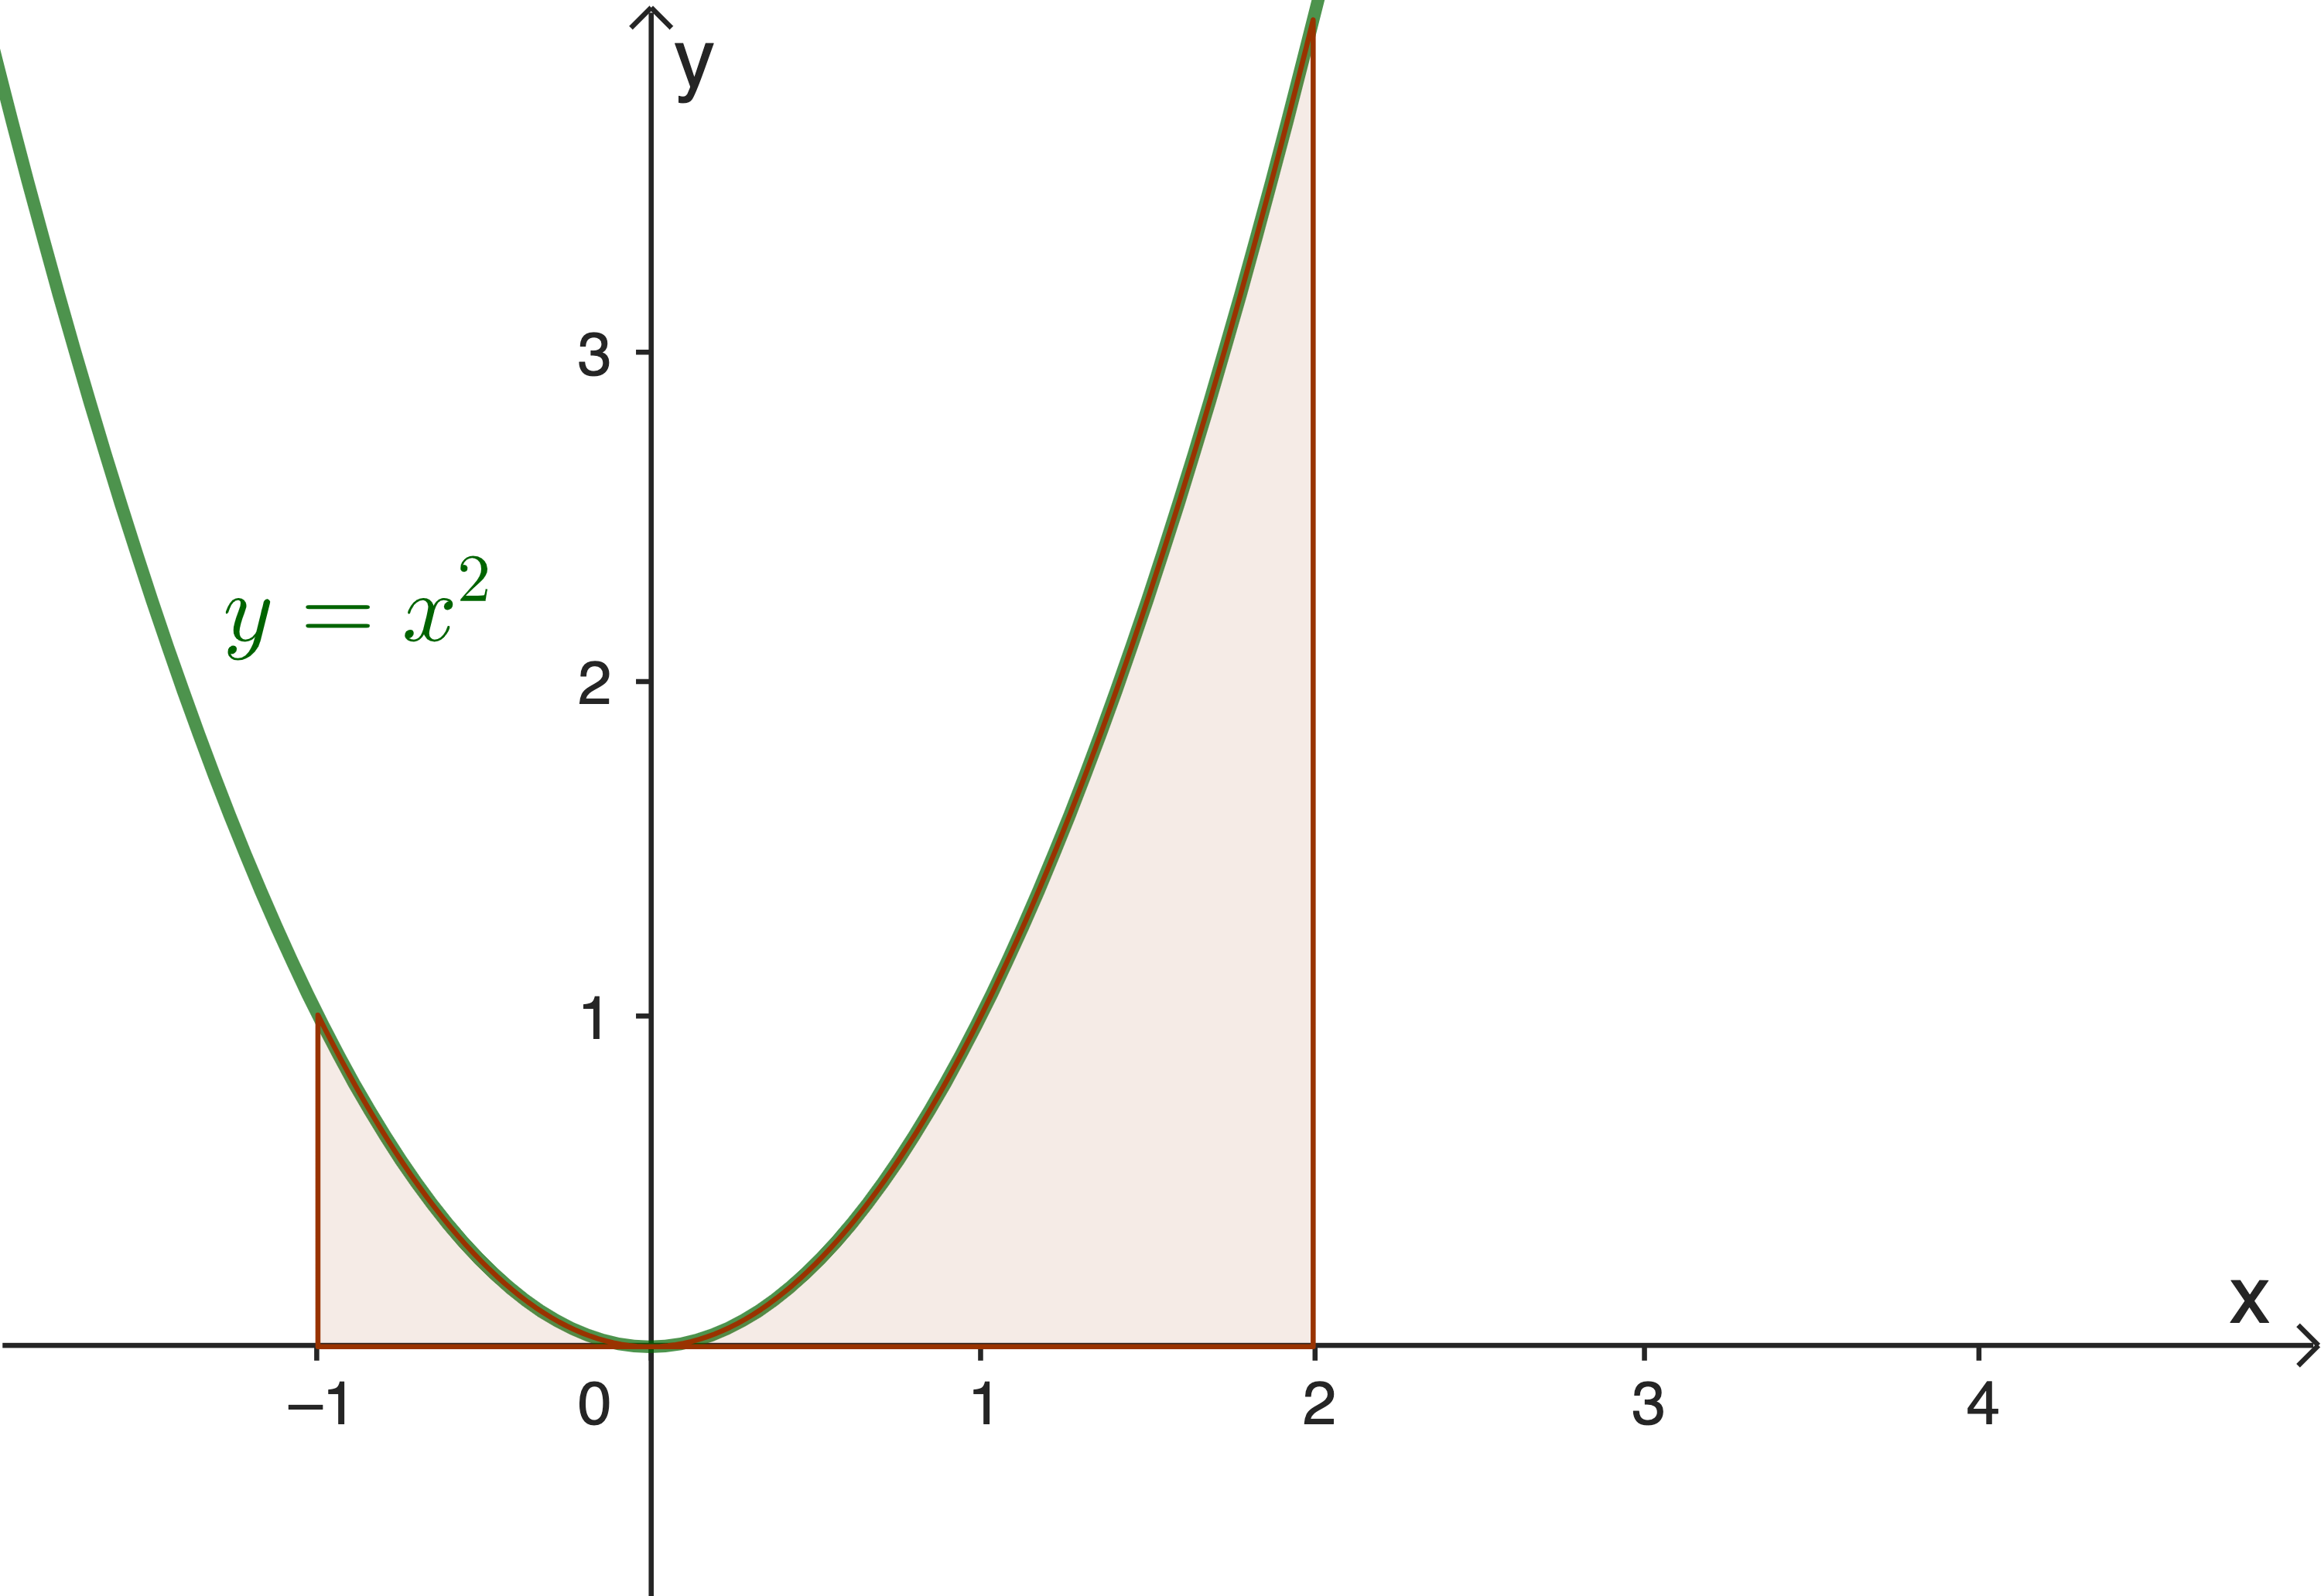
\includegraphics[width = 0.25\textwidth]{media/integral--1-2-xquadrat.png}
\end{center}

Freilich wäre jede dieser Rechnung mit Aufwand verbunden. Einfacher geht es, wenn man das rechte Ende des Intervalls variabel lässt.

Betrachten Sie die Fläche unter dem Graphen von $f(x)=x^2$ im Intervall $[0,b]$:
\begin{center}
	\includegraphics[width=0.5\textwidth]{media/flächeUnterxQuadrat.png}
\end{center}

In der folgenden Lernaufgabe werden wir eine Funktion $F(b)$ herleigen, die in Abhängigkeit von $b$ den Inhalte der Fläche unter der Parabel $y=x^2$ im Intervall $[0, b]$ berechnet. (Eine solche Funktion nennt man eine \emph{Integralfunktion} von $f$)


% Idee: Zur Bestimmung des Flächeninhalts unter der Parabel teilen wir das Intervall $[0,b]$ in vier Teile und betrachten zwei Näherungen für den Flächeninhalt:

% Die Summe der Flächeninhalte der 4 Rechtecke in der Figur links nennen wir \textbf{Untersumme} $U_4$.(Beachten Sie, dass es ganz links ein \glqq Rechteck\grqq{} mit der Höhe 0 gibt)
% \begin{center}
% 	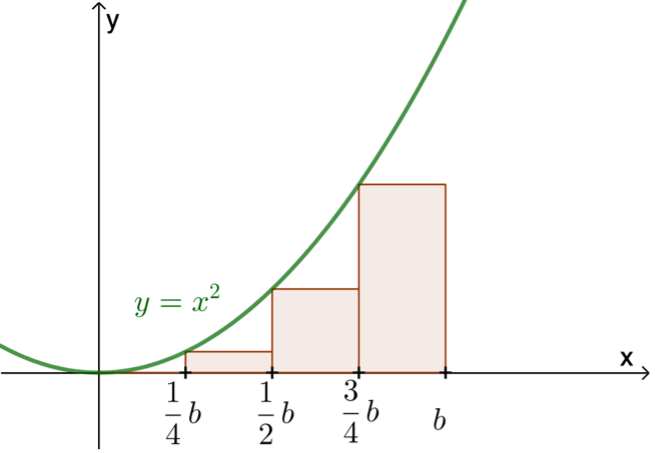
\includegraphics[width=0.5\textwidth]{media/UntersummexQuadrat.png}
% \end{center}

% Die Summe der Flächeninhalte der 4 Rechtecke in der Figur rechts nennen wir \textbf{Obersumme} $O_4$.

% \begin{center}
% 	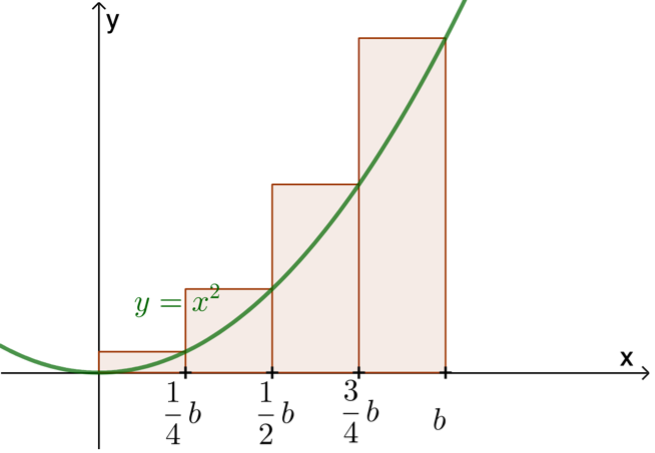
\includegraphics[width=0.5\textwidth]{media/ObersummexQuadrat.png}
% \end{center}
\begin{LA}
	{Die Fläche unter der Quadratfunktion - Teil 2}{FlächeUnterxQuadrat-teil2}
	\begin{enumerate}
		\item Gehen Sie wie in \Cref{LA:FlächeUnterxQuadrat-teil1} vor, um die Fläche unter der Parabel $y=x^2$ im Intervall $[0,b]$ zu berechnen. Berechnen Sie also die Untersumme $U_n$ und die Obersumme $O_n$ für eine Zerlegung des Intervalls in $n$ Teile. Verwenden Sie die Summenformel, um die Terme zu vereinfachen und bestimmen Sie den Grenzwert von $U_n$ und $O_n$ für $n\rightarrow \infty$.
		\item Berechnen Sie mit der Formel die Fläche unter der Parabel $y=x^2$ in den Intervallen $[0,2]$, [1,2] und $[-1,2]$ (Siehe die drei Abbildungen oben).

	\end{enumerate}
\end{LA}































\clearpage
\subsubsection{Ober- und Untersummen}

\begin{satz}
	{Erkenntnis aus der Lernaufgabe}{}
	Der Inhalt der Fläche zwischen der Parabel $y=x^2$ und der $x$-Achse im Intervall $[0,b]$ beträgt
	$$ A=\frac{1}{3} b^3$$
	\begin{center}
		\includegraphics[width=0.5\textwidth]{media/flächeUnterxQuadrat.png}
	\end{center}
\end{satz}


\begin{proof}
	Teilt man das Intervall $[0,b]$ in $n$ Teilintervalle erhält man die Untersumme
	\begin{align*}
		U_n & = \frac{b}{n} \left[f\left(\frac{b}{n} \right)+f\left(\frac{2b}{n} \right)+f\left(\frac{3b}{n} \right)+\cdots +f\left(\frac{(n-1)b}{n} \right)\right] \\
		    & =\frac{b}{n} \left[ \frac{b^2}{n^2} +\frac{4b^2}{n^2} + \frac{9b^2}{n^2} + \cdots +\frac{(n-1)^2 b^2}{n^2} \right]                                    \\
		    & = \frac{b^3}{n^3} \left[1+4+9+\cdots+(n-1)^2 \right]
	\end{align*}

	Analog für die Obersumme:
	$$ O_n=\frac{b^3}{n^3}  [1+4+9+\cdots +n^2 ]$$
	Nun verwenden wir die Formel für die Summe der Quadratzahlen.
	$$ 1+4+9+16+\cdots +k^2=\frac{k(k+1)(2k+1)}{6} $$
	Damit folgt für $k=n-1$:
	$$ U_n= \frac{b^3}{n^3} \left[ \frac{(n-1)n(2n-1)}{6} \right] =  \frac{b^3}{6} \cdot  \frac{2n^2-3n+1}{n^2} = \frac{b^3}{6} \left(2-\frac{3}{n}+\frac{1}{n^2}\right)
	$$
	Und für $k=n$:
	$$ O_n= \frac{b^3}{n^3} \left[ \frac{n(n+1)(2n+1)}{6} \right] =  \frac{b^3}{6} \cdot \frac{2n^2+3n+1}{n^2} = \frac{b^3}{6} \left(2+\frac{3}{n}+\frac{1}{n^2}\right)
	$$
	Der Grenzwert von Ober- und Untersumme beträgt schliesslich:
	$$ \lim_{n\rightarrow\infty} U_n = \lim_{n\rightarrow\infty} O_n = \frac{b^3}{6}\cdot 2 = \frac{b^3}{3}  $$
\end{proof}

% \begin{ueb}{}{}
%     \begin{enumerate}
%         \item  Benutzen Sie die Formel für die Fläche unter der Parabel, um folgende Flächeninhalte zu berechnen.
%         \begin{enumerate}
%             \item Fläche zwischen der $x$-Achse und dem Graphen von $f(x)=x^2$ zwischen $x=0$ und $x=5$.
%             \item Fläche zwischen der $x$-Achse und dem Graphen von $f(x)=x^2$ zwischen $x=3$ und $x=6$.
%             \item Fläche zwischen der $x$-Achse und dem Graphen von $f(x)=x^2+3$ zwischen $x=0$ und $x=2$. Tipp: machen Sie eine Skizze und unterteilen Sie die Fläche in zwei Teile, deren Inhalt Sie berechnen können.
%             \item Fläche zwischen der $x$-Achse und dem Graphen von $f(x)=5\cdot x^2$ zwischen $x=0$ und $x=6$. Tipp: Wie verändern sich die Rechtecke in Unter- und Obersumme, wenn man anstatt $y=x^2$ die Kurve $y=5x^2$ betrachten?
%         \end{enumerate}
%     \item Lösen Sie die Aufgaben auf Seite 124 - 128 im Buch. Beispielsweise 34, 36 und 39.
%     \end{enumerate}
%   
%\end{ueb}

Das Verfahren, das wir für die Funktion $y=x^2$ verwendet haben, lässt sich auch auf andere Funktionen übertragen.
\begin{definition}
	{Ober- und Untersumme}{}
	Sei $f$ eine stetige Funktion $f:\,   [a,b]\rightarrow \R$. Wir unterteilen das Intervall $[a,b]$ in $n$ gleich grosse Teilintervalle $[x_{k-1} x_{k}]$ der Breite $ \Delta x = \frac{b-a}{n}$.
	\bigskip



	\textbf{Untersumme $U_n$:} \\
	\begin{center}
		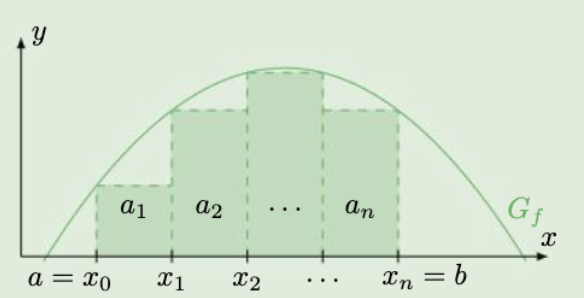
\includegraphics[width = 0.3\textwidth]{media/UntersummeDef.png}
	\end{center}
	Für jedes Teilintervall wählen wir den kleinsten Funktionswert $\underline{f_k}$.
	%$\underline{f_k} = \min \{ f(x) | x\in [x_{k-1}, x_{k}] \}$
	Die Untersumme $U_n$ ist definiert als die Summe der Flächeninhalte $a_k = \Delta x \cdot \underline{f_k}$ der Rechtecke mit der Breite $\Delta x$ und der Höhe $\underline{f_k}$:
	$$U_n = a_1 +  a_2 + \cdots +a_n = \sum_{k=1}^n \underline{f_k} \cdot \Delta x $$


	\bigskip

	\textbf{Obersumme $O_n$:} \\
	\begin{center}
		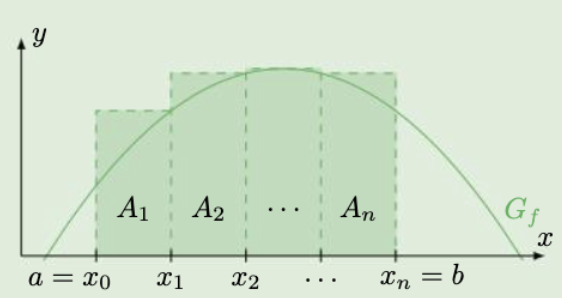
\includegraphics[width = 0.3\textwidth]{media/ObersummeDef.png}
	\end{center}
	Für jedes Teilintervall wählen wir den grössten Funktionswert $\overline{f_k}$.
	%$\underline{f_k} = \max \{ f(x) | x\in [x_{k-1}, x_{k}] \}$
	Die Obersumme $O_n$ ist definiert als die Summe der Flächeninhalte $a_k = \Delta x \cdot \overline{f_k}$ der Rechtecke mit der Breite $\Delta x$ und der Höhe $\overline{f_k}$:
	$$O_n = A_1 +  A_2 + \cdots +A_n = \sum_{k=1}^n \overline{f_k} \cdot \Delta x $$






	% \begin{center}
	%     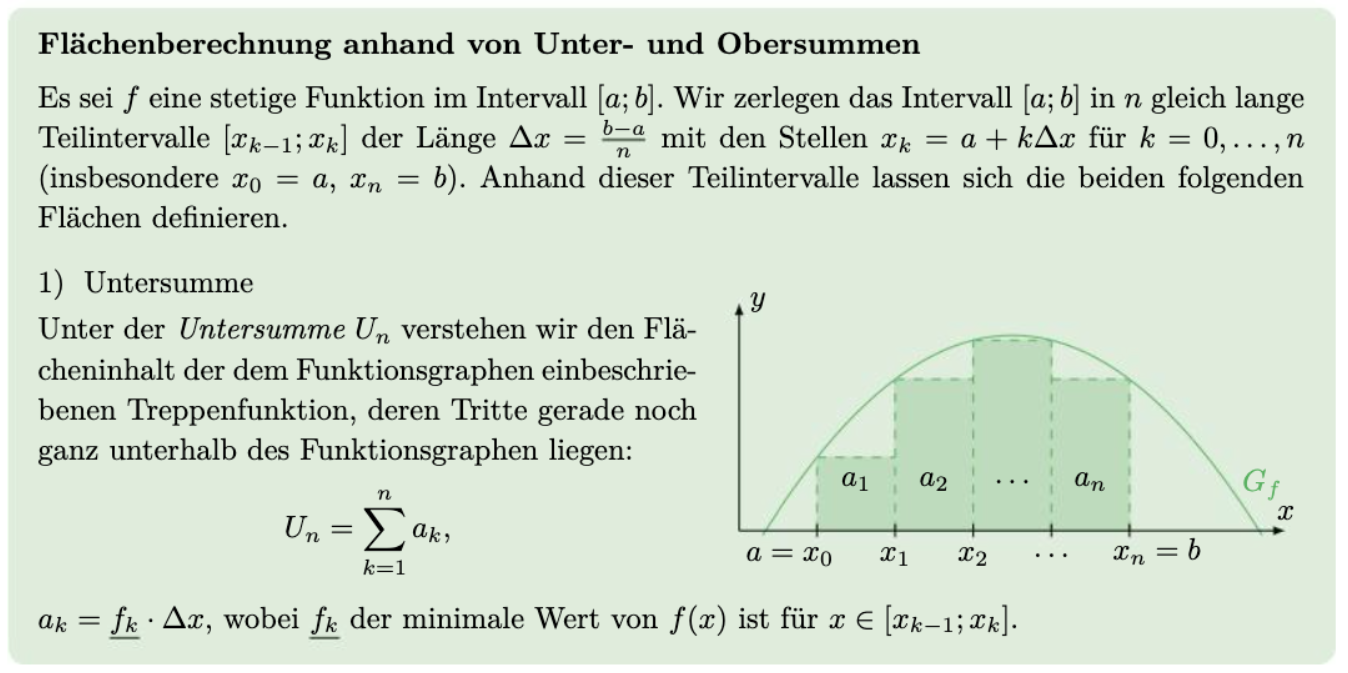
\includegraphics[width = \textwidth]{media/defUntersumme.png}

	%     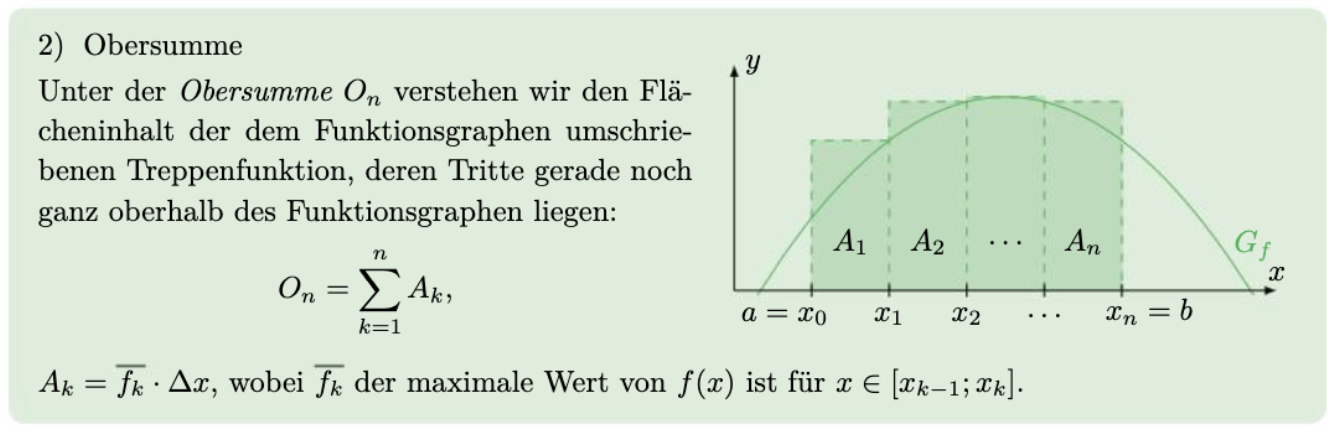
\includegraphics[width = \textwidth]{media/defObersumme.png}
	% \end{center}


\end{definition}

\clearpage
\begin{ueb}
	{Fläche unter einer Funktion dritten Grades}{}


	\begin{enumerate}
		\item Die Abbildung zeigt den Grundriss eines Schwimmbeckens, dessen Breite alle 2m gemessen wurde. Schätzen Sie den Flächeninhalt des Beckens mit Hilfe von Unter- und Obersummen ab.
		      \begin{center}
			      \includegraphics[width = 0.3\textwidth]{media/SchwimmbeckenFläche.png}
		      \end{center}


		\item
		      In dieser Aufgabe sollen Sie die Fläche unter dem Graphen der Funktion $f(x) = \frac{1}{100} x^3$ im Intervall $[0,10]$ untersuchen.
		      Tipp: Der Taschenrechner TI 30 X Pro kann mit Summenzeichen umgehen. Siehe dieses \href{https://youtu.be/rxhaYyTZ25o}{Anleitungsvideo}.

		      \begin{enumerate}
			      \item Berechnen Sie die Untersumme $U_5$ und die Obersumme $O_5$.
			      \item Berechnen Sie die Untersumme $U_{10}$ und die Obersumme $O_{10}$.
			      \item Bestimmen Sie je einen Term für die Unter- bzw. Obersumme $U_n$ bzw. $O_n$, wenn man das Intervall in $n$ Teile unterteilt.
			            Dazu können Sie die Formel für die Summe der Kubikzahlen verwenden:
			            $$ 1^3 + 2^3 + 3^3 + \cdots + k^3 = \left( \frac{k(k+1)}{2} \right)^2 $$
			      \item Welchen Grenzwert erhält man für die beiden Summen, für $n \rightarrow \infty$?
		      \end{enumerate}
	\end{enumerate}
\end{ueb}


\clearpage
\emph{Lösungen:}
\begin{enumerate}
	\item Schwimmbecken:

	      Untersumme $U = 55 m^2$; \quad Obersumme $O = 83.8 m^2$. Die echte Fläche liegt also zwischen diesen beiden Werten.
	\item Fläche unter kubischer Funktion
	      \begin{enumerate}
		      \item $U_5= 16,\quad O_5 = 36$
		      \item $U_{10} = 20.25,\quad O_{10} = 30.25$
		      \item $U_n = 25\left(1-\frac{1}{n}\right)^2; \quad O_n = 25\left(1+\frac{1}{n}\right)^2$
		      \item $\lim_{n\rightarrow\infty} U_n = \lim_{n\rightarrow\infty} O_n = 25$
	      \end{enumerate}

\end{enumerate}

\newpage












\subsubsection{Das bestimmte Integral und Integralfunktionen}


\begin{definition}
	{Das bestimmte Integral}{}
	% 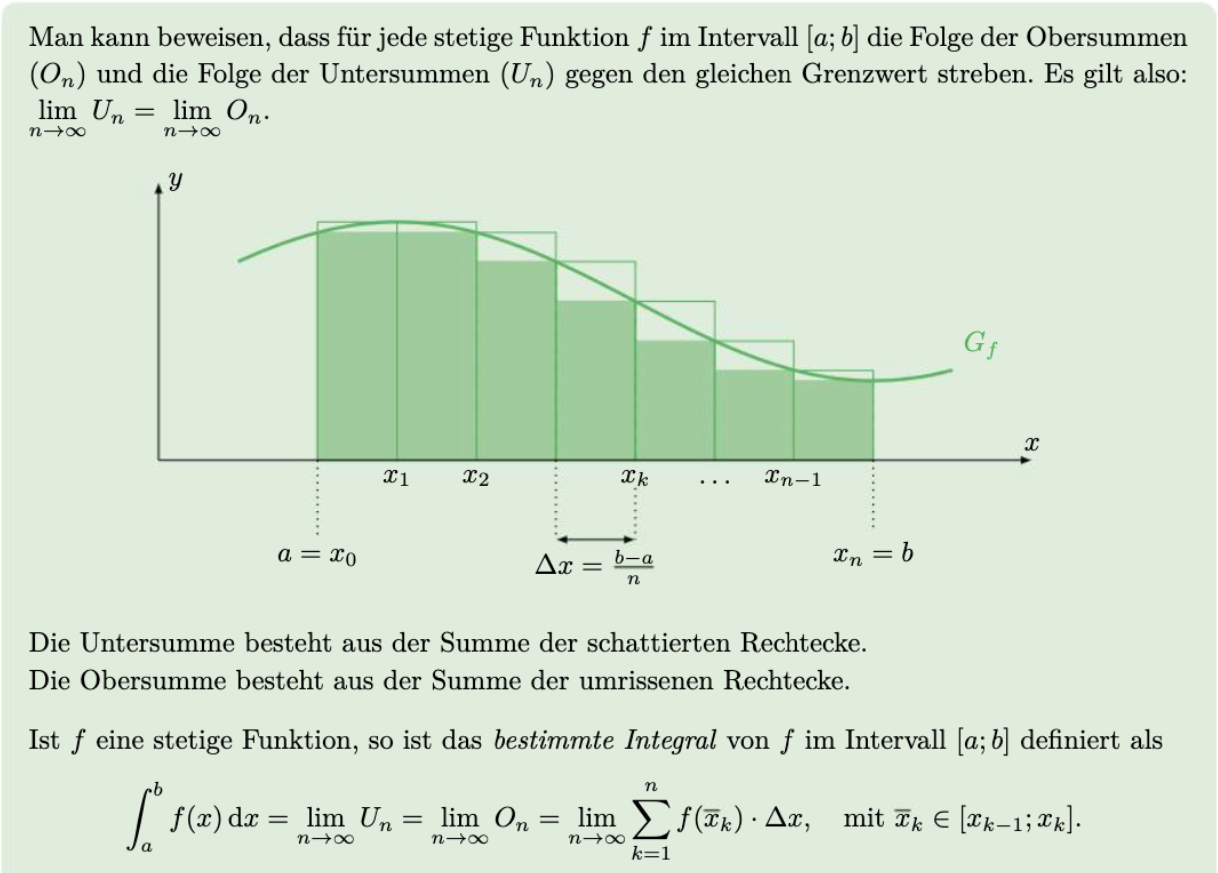
\includegraphics[width = \textwidth]{media/defBestInt-1.png}
	% 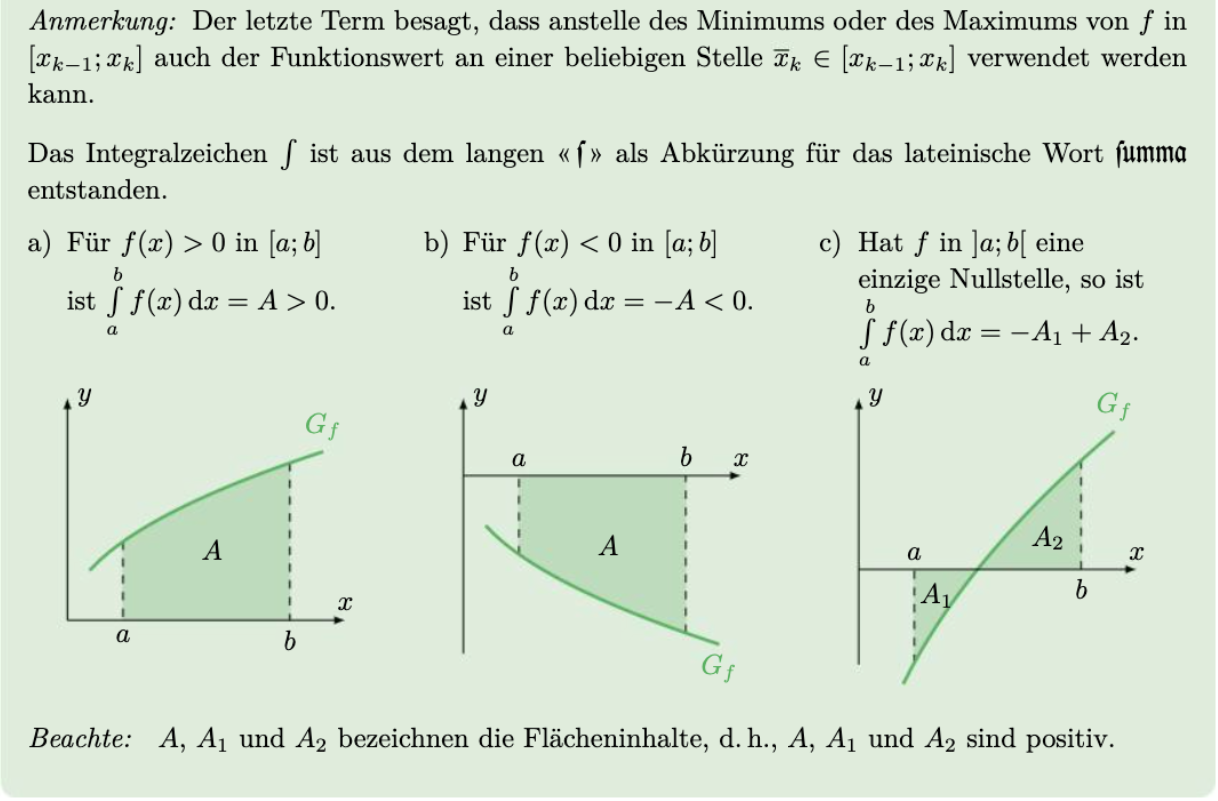
\includegraphics[width = \textwidth]{media/defBestInt-2.png}
	Sei $f$ eine Funktion $f:\,   [a,b]\rightarrow \R$. Falls Unter- und Obersumme den gleichen Grenzwert besitzen $\lim_{n\rightarrow\infty} U_n = \lim_{n\rightarrow\infty} O_n$, so sagt man, die Funktion $f$ sei \emph{integrierbar}. Den gemeinsamen Grenzwert von Ober- und Untersumme nennt man das \emph{bestimmte Integral der Funktion $f$ von $a$ nach $b$}.

	Schreibweise
	$$ \int_a^b f(x) dx =  \lim_{n\rightarrow\infty} U_n = \lim_{n\rightarrow\infty} O_n$$

	Wenn die Funktion $f$ im Intervall $[a,b]$ nicht negativ ist, entspricht das bestimmte Integral dem Flächeninhalt des Gebietes, das durch den Graphen von $f$, die $x$-Achse und die Geraden $x=a$ und $x=b$ berandet wird. Weil aber die Flächeninhalte der Rechtecke in Ober- und Untersumme berechnet werden mit $a_= \Delta x \cdot \underline{f_k}$ bzw. $A_k = \Delta x \cdot \overline{f_k}$, kann das bestimmte Integral auch negative Werte annehmen, wenn die Funktion im Intervall negative Funktionswerte annimmt.
	\begin{center}
		\includegraphics[width = \textwidth]{media/flächenbilanz.png}
	\end{center}




\end{definition}


\begin{bsp}
	{}{}
	In der Lernaufgabe am Anfang des Kapitels haben wir gezeigt, dass der Inhalt der Fläche zwischen der Parabel $y=x^2$ und der $x$-Achse im Intervall $[0,b]$  $ A=\frac{1}{3} b^3$ beträgt. In anderen Worten:
	$$ \int_0^b x^2 dx = \frac{1}{3} b^3$$
	Mit dieser Formel können wir nun verschiedene bestimmte Integrale berechnen:
	\begin{itemize}
		\item $\int_0^5 x^2 dx = \frac{1}{3} 5^3 = \frac{125}{3}$
		\item $\int_1^3 x^2 dx = \int_0^3 x^2 dx - \int_0^1 x^2 dx = \frac{1}{3} 3^3 -\frac{1}{3} 1^3 = \frac{26}{3}$
	\end{itemize}
	\begin{center}
		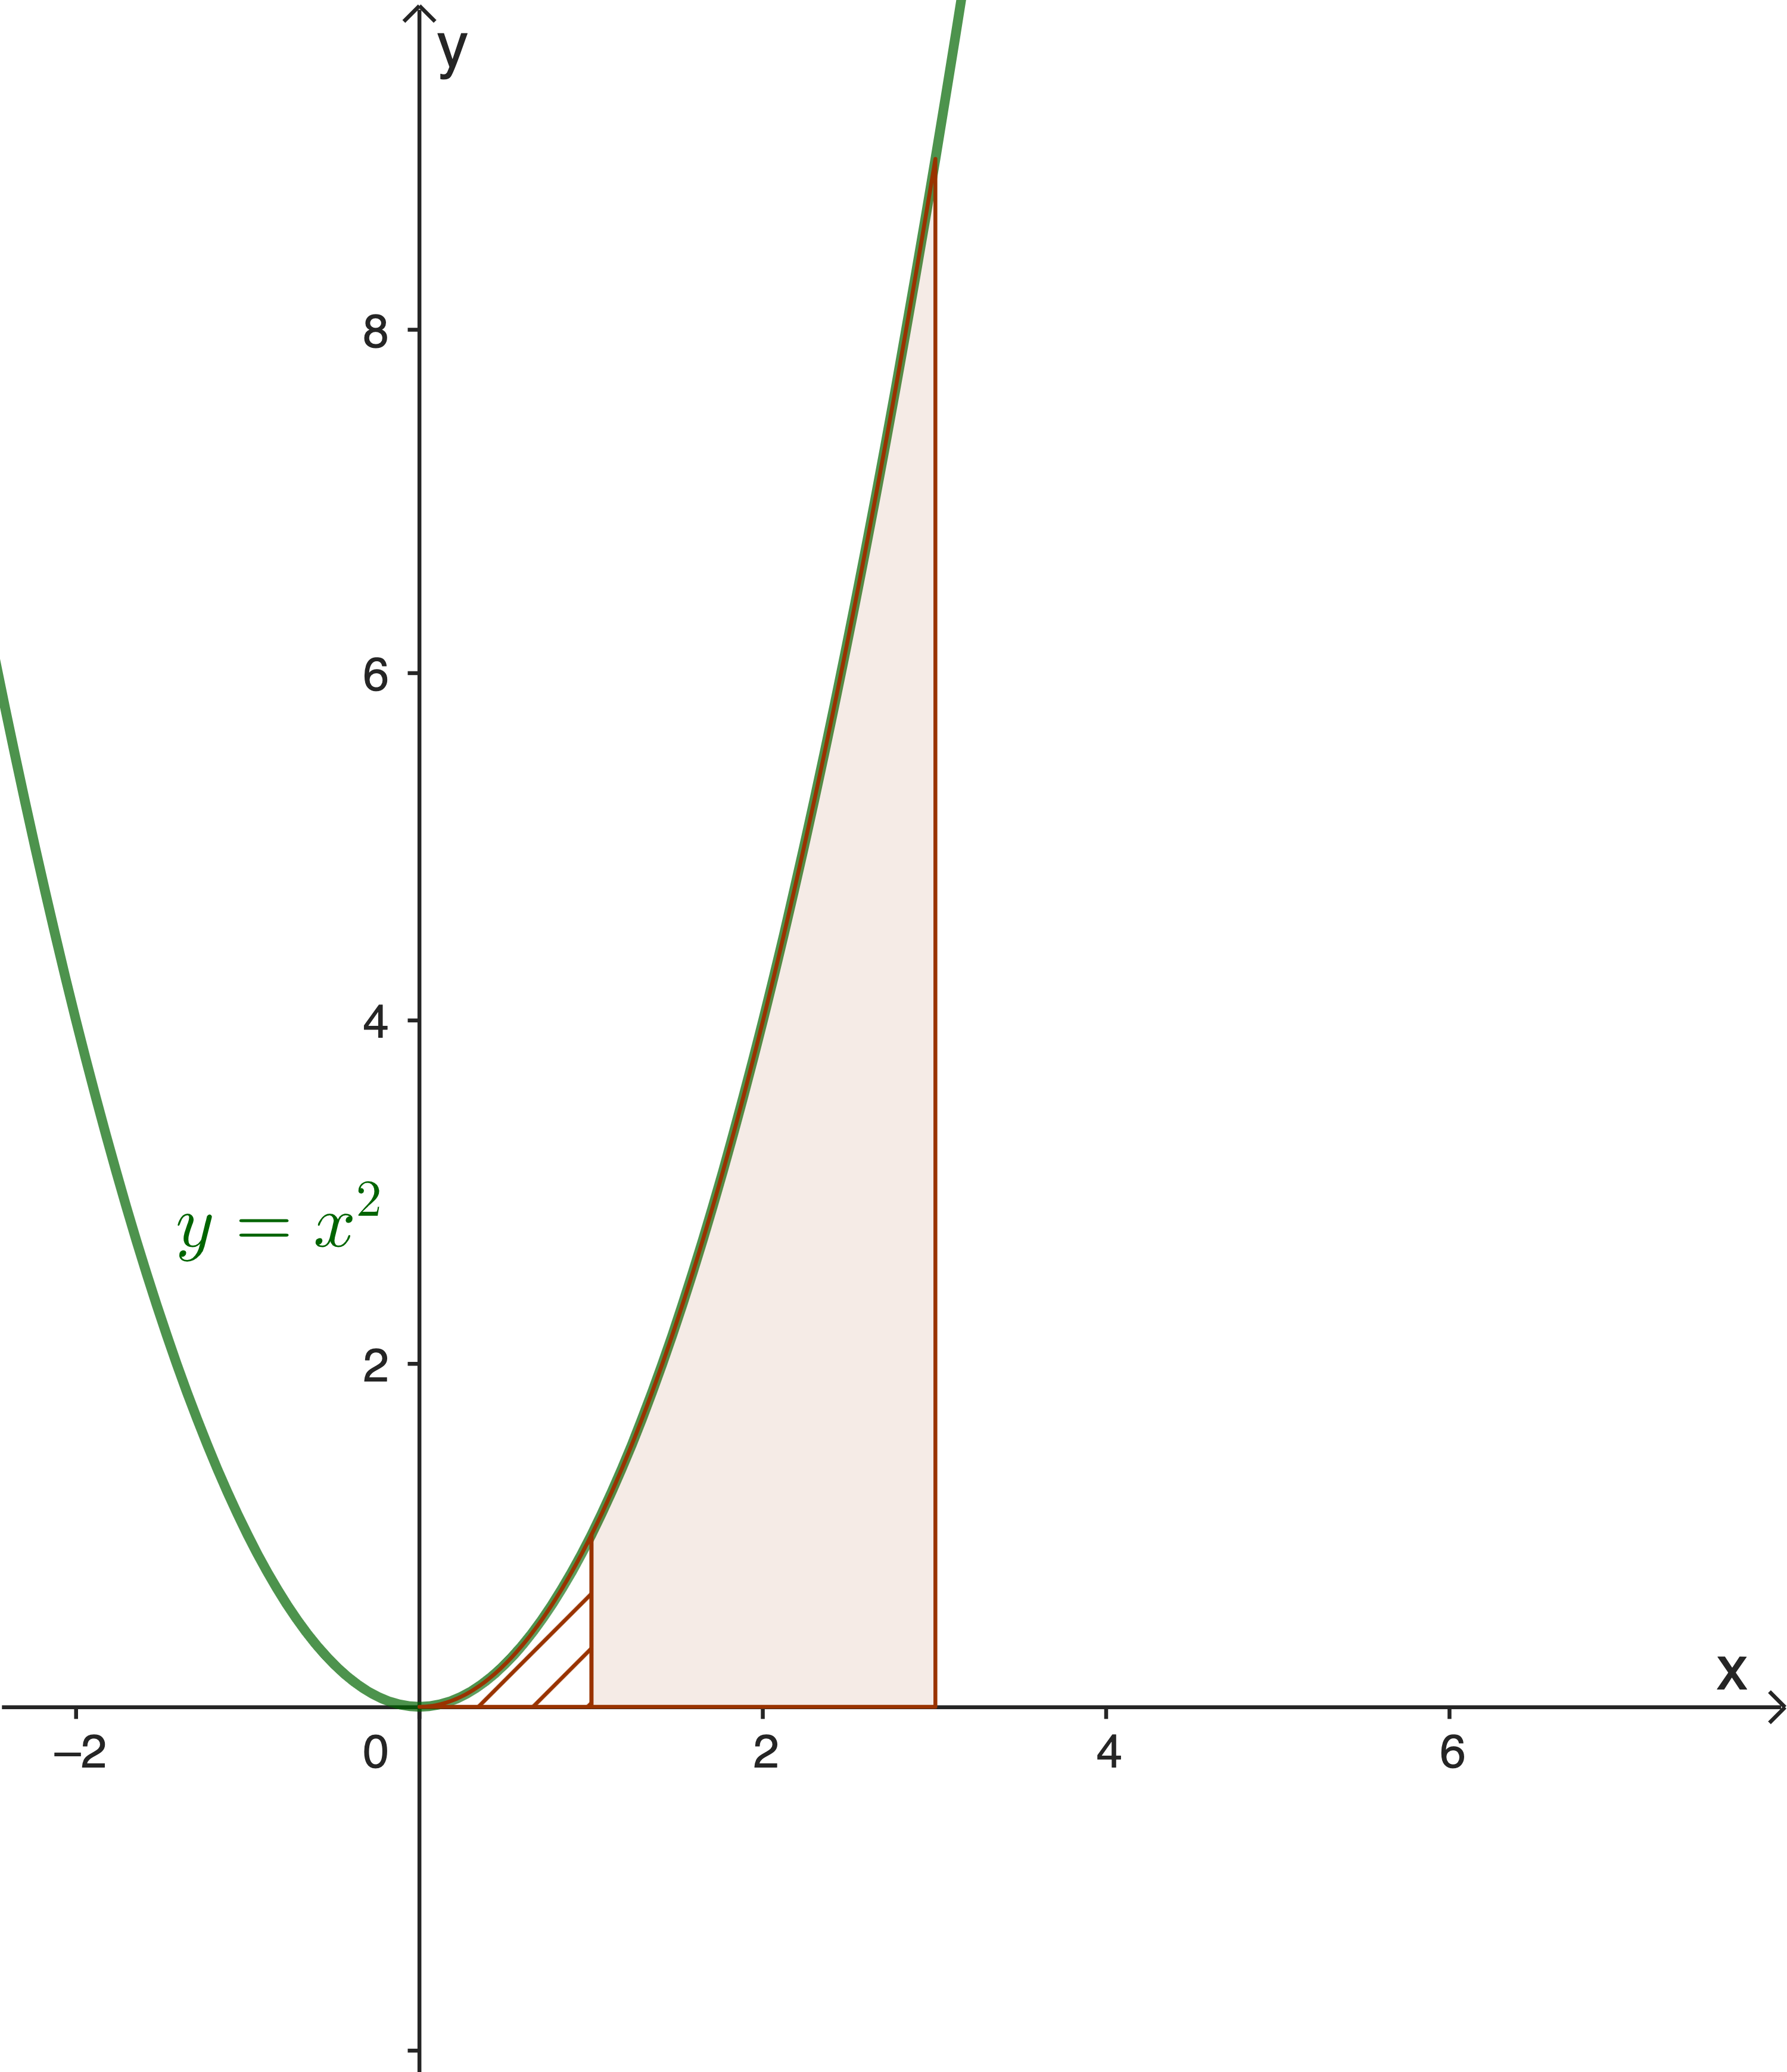
\includegraphics[width = 0.5\textwidth]{media/integral1-3.png}
	\end{center}
\end{bsp}
Beim zweiten Beispiel haben wir intuitiv die erste der folgenden Integrationsregeln verwendet:
\begin{satz}
	{Aufteilen und Vertauschen der Integrationsgrenzen }{}
	$$\int_a^b f(x) dx + \int_b^c f(x) dx = \int_a^c f(x) dx $$
	$$\int_b^a f(x) dx  = - \int_a^b f(x) dx $$
\end{satz}
Um die zweite Regel zu verstehen, muss man einen Blick zurück auf die Definition der Untersummen werfen:
$$U_n = \sum_{k=1}^n \underline{f_k} \cdot \Delta x, $$
wobei $\Delta x = \frac{b-a}{n}$ die Breite der Rechtecke ist.

Wenn die beiden Integrationsgrenzen vertauscht werden, ändert sich in der ganzen Summe bloss das Vorzeichen im Zähler von $\Delta x$.

In der Lernaufgabe am Anfang des Kapitels haben wir die Formel $$ \int_0^b x^2 dx = \frac{1}{3}b^3$$ hergeleitet. Weil wir die obere Grenze des Integrals variabel gelassen haben, kann man mit dieser Formel in Kombination mit dem Aufteilen der Integrationsgrenzen alle bestimmte Integrale rund um die Funktion $f(x)=x^2$ berechnen. So gilt zum Beispiel:

$$\int_5^{10} x^2 dx = \int_0^{10} x^2 dx - \int_0^5 x^2 dx = \frac{1}{3}10^3-\frac{1}{3}5^3 = \frac{875}{3}$$

Diese Idee lässt sich auf andere Funktionen übertragen:
\begin{definition}{Integralfunktion}{}
	Sei $f$ eine stetige Funktion. Die Integralfunktion von $f$ zur unteren Grenze $a$ ist definiert als:
	$$F_a (b) = \int_a^b f(x) dx$$
\end{definition}
Bemerkung: Die untere Grenze $a$ des Integrals ist hier fest gewählt, während die obere Grenze $b$ variabel ist.
\begin{bsp}
	{Integralfunktion der Quadratfunktion zur unteren Grenze $0$}{}
	Sei $f(x)=x^2$. Die Erkenntnis aus der Lernaufgabe am Anfang des Kapitels lautet dann:
	$$F_0(b)=\frac{1}{3} b^3$$
\end{bsp}
% \clearpage
\begin{ueb}
	{}{}


	\begin{enumerate}
		\item Für die Funktion \(f\) gilt:
		      \[
			      \int_{-1}^{1} f(x)\,dx = -2
			      \quad\text{und}\quad
			      \int_{1}^{4} f(x)\,dx = 5.
		      \]
		      Berechnen Sie die vier Integrale.

		      \begin{enumerate}
			      \item \(\displaystyle \int_{4}^{1} f(x)\,dx\)
			      \item \(\displaystyle \int_{-1}^{4} f(x)\,dx\)
			      \item \(\displaystyle \int_{1}^{1} f(x)\,dx\)
			      \item \(\displaystyle \int_{-1}^{1} 4 \cdot f(x)\,dx\)
		      \end{enumerate}
		\item Der Graph \(G_f\) der Funktion \(f\) ist gegeben.
		      \begin{center}
			      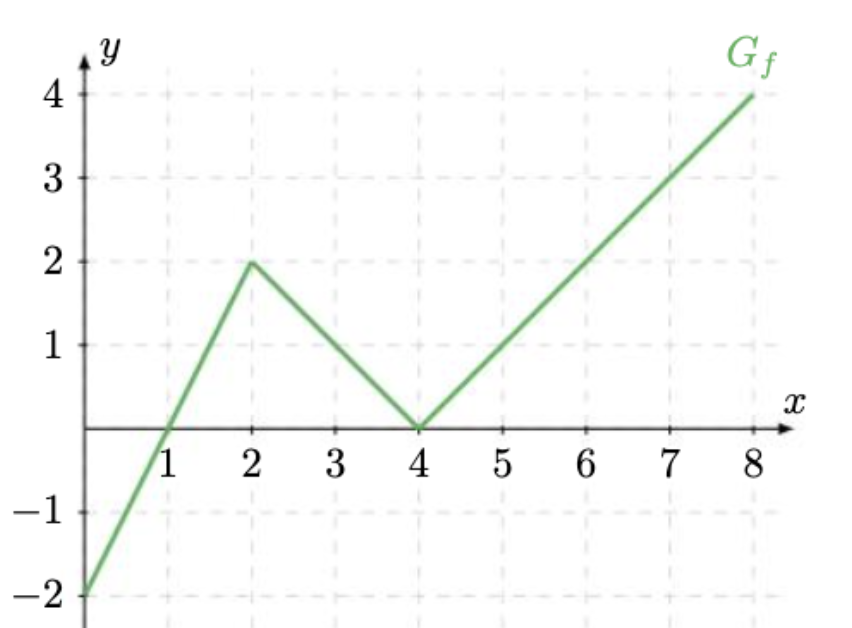
\includegraphics[width = 0.3 \textwidth]{media/GraphAufgabe45.png}
		      \end{center}

		      \begin{enumerate}
			      \item Bestimmen Sie \(\displaystyle \int_{1}^{7} f(x)\,dx.\)
			      \item Bestimmen Sie \(\displaystyle \int_{0}^{1} f(x)\,dx.\)
			      \item Bestimmen Sie \(\displaystyle \int_{0}^{7} f(x)\,dx.\)
			      \item Berechnen Sie den Inhalt der Fläche, die der Graph \(G_f\) im Intervall \([0,7]\) mit der \(x\)-Achse einschliesst.
		      \end{enumerate}

		\item Skizzieren Sie den Graphen der folgenden Funktionen. Markieren Sie in der Skizze die Fläche mit dem Inhalt  \(F_0(b) = \int_0^b f(x) \, dx\) (mit \(b \ge 0\)).

		      Geben Sie anschliessend eine Formel für den Inhalt der markierten Fläche an.

		      %   Bestimme jeweils die Funktionsgleichung der Integralfunktion \(F_0(b) = \int_0^b f(x) \, dx\) (mit \(b \ge 0\)) der folgenden
		      %   Funktion \(f\).

		      %   \textit{Tipp:} Es handelt sich hier immer um lineare Funktionen, weshalb sich die Integralfunktion
		      %   anhand des Funktionsgraphen durch geometrische Überlegungen bestimmen lässt.

		      \begin{enumerate}
			      \item \(f(x) = 1\)
			      \item \(f(x) = 2\)
			      \item \(f(x) = c,\; c \in \mathbb{R}_0^{+}\)
			      \item \(f(x) = x\)
			      \item \(f(x) = 2x\)
			      \item \(f(x) = mx,\; m \in \mathbb{R}_0^{+}\)
			      \item \(f(x) = x + 1\)
			      \item \(f(x) = 2x + 1\)
			      \item \(f(x) = mx + q,\; m,c \in \mathbb{R}_0^{+}\)
		      \end{enumerate}


	\end{enumerate}
\end{ueb}
\clearpage

\emph{Lösungen}

\begin{enumerate}
	\item Integrale Berechnen
	      \begin{enumerate}
		      \item -5
		      \item 3
		      \item 0
		      \item -8
	      \end{enumerate}
	\item Graph
	      \begin{enumerate}
		      \item 7.5
		      \item -1
		      \item 6.5
		      \item 8.5
	      \end{enumerate}
	\item Integralfunktionen
	      \begin{enumerate}
		      \item $F_0(b) = b$
		      \item $F_0(b) = 2b$
		      \item $F_0(b) = c\cdot b$
		      \item $F_0(b) = \frac{1}{2} b^2$
		      \item $F_0(b) = b^2$
		      \item $F_0(b) = \frac{m}{2} b^2$
		      \item $F_0(b) = \frac{1}{2} b^2 + b$
		      \item $F_0(b) = b^2 + b$
		      \item $F_0(b) = \frac{m}{2} b^2 + q\cdot b$
	      \end{enumerate}
\end{enumerate}